%This is chapter 4
%%=========================================
\chapter[Results]{Results}
To test the validity of the implementation a series of slope stability simulations is run.
The results from these simulations is presented in the following sections.


\section{Slope Stability problem - Homogeneous isotropic soil - Zero variance}

To check the base case of spatially invariant soil with known analytical solutions. This is to validate the input to the random field generation, the FEM mesh and calculation. The simulation is a elasto-plastic FEM simulation with Mohr-Couloumb material model using Plaxis undraind(C) behaviour. 15-Node triangular FEM elements are used. The slope is 5 meter high with a 2:1 gradient.
The soil parameters is presented in Table \ref{tab1}. The resulting random field, or in this particular case a constant field, is shown in Figure \ref{fig:p1} and the 2:1 slope geometry and Plaxis 2D mesh is shown in Figure \ref{fig:p2}.


\begin{table}[h]
	\centering\small
	\caption{Soil parameters for Homogeneous isotropic soil}
	\label{tab1}
		\begin{tabular*}{\textwidth}{@{\extracolsep{\fill}}lccc}
			\toprule
			 Soil model  &\multicolumn{3}{c}{Mohr Couloumb - Undrained(C)}\\
  \cmidrule{2-4}
			Statistical Soil	& Mean		 	& Coefficient of Variation 		& Scale of fluctuation \\
			Parameters	  	& $\mu$ 		&  $CoV = \frac{\sigma}{\mu}$ 		& $\theta$ \\
        
			\midrule
			  Unit weight, $\gamma_{sat}=\gamma{unsat}$ & 20 $kN/m^3$ & 0 & - \\
		          Modulus of elasticity, $E$ & 10 $MPa$ & 0 & - \\
		          Poissons ratio, $\nu$ & 0.49 & 0 & - \\
		          Undrained Shear Strength,$S_u$ & 20 $kPa$ & 0 & - \\
			\bottomrule
		\end{tabular*}
\end{table}

Running a Plaxis c-reduction calculation phase, result graph plotted in \ref{fig:psf1}, on the uniform soil slope gives a Factor of Safety, $F_s = 1.14$. The corresponding $F_s$ obtained by slope stability charts after \citet{Janbu1968slope} is $F_s = 1.16$. 

\begin{figure}[h]
	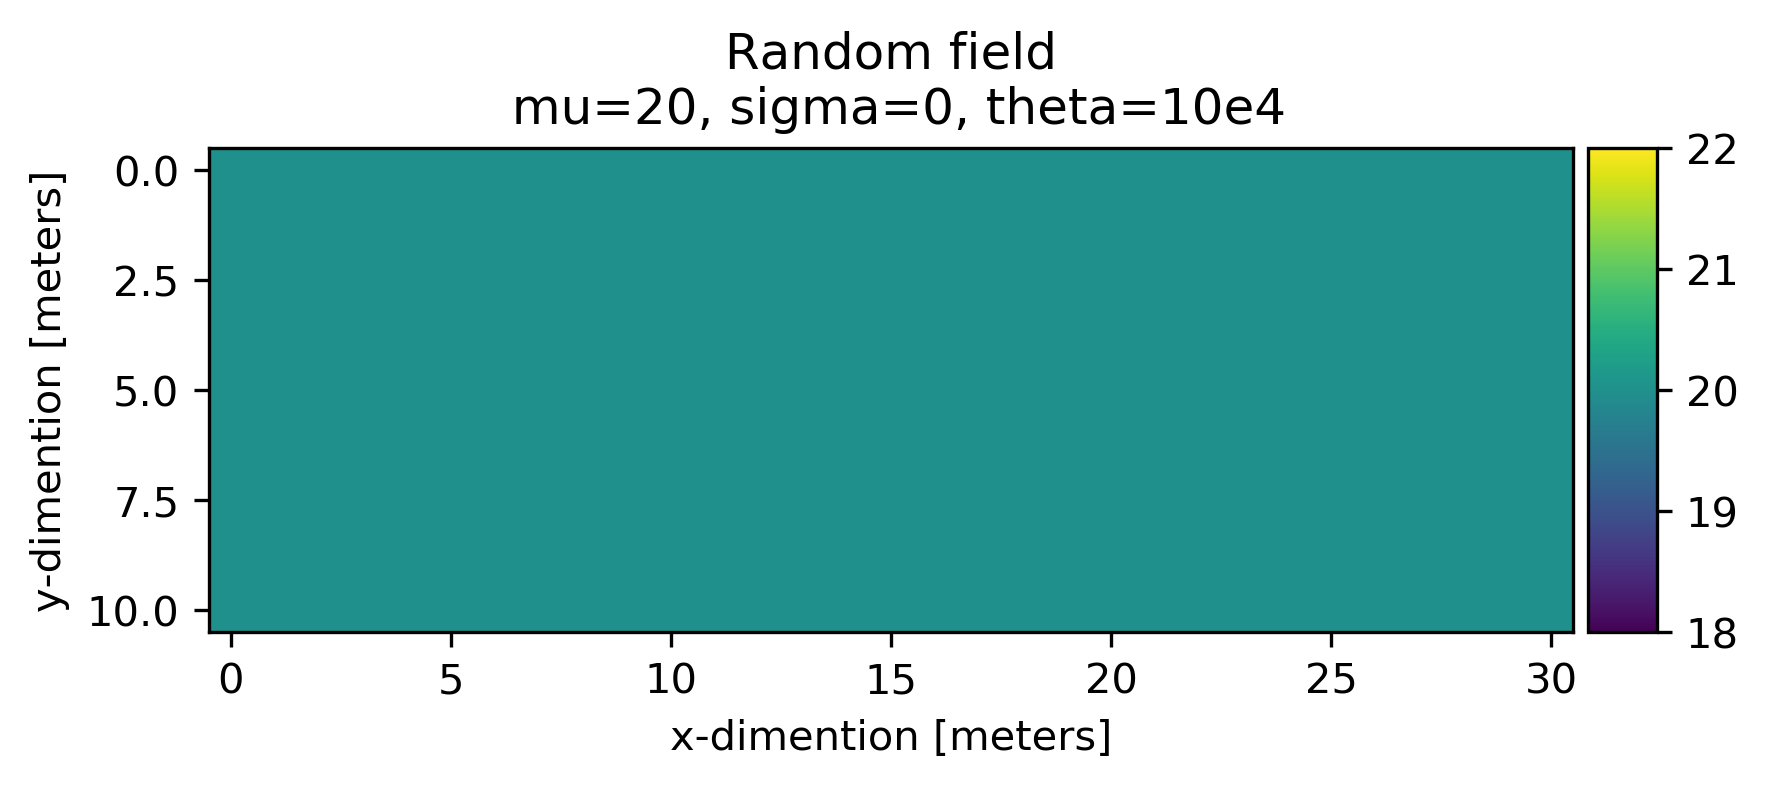
\includegraphics[width=\textwidth]{fig/testRF}
	\caption{$S_u$ Random field, in this particular case the soil strength is uniform}
	\label{fig:p1}
\end{figure}

\begin{figure}[h]
	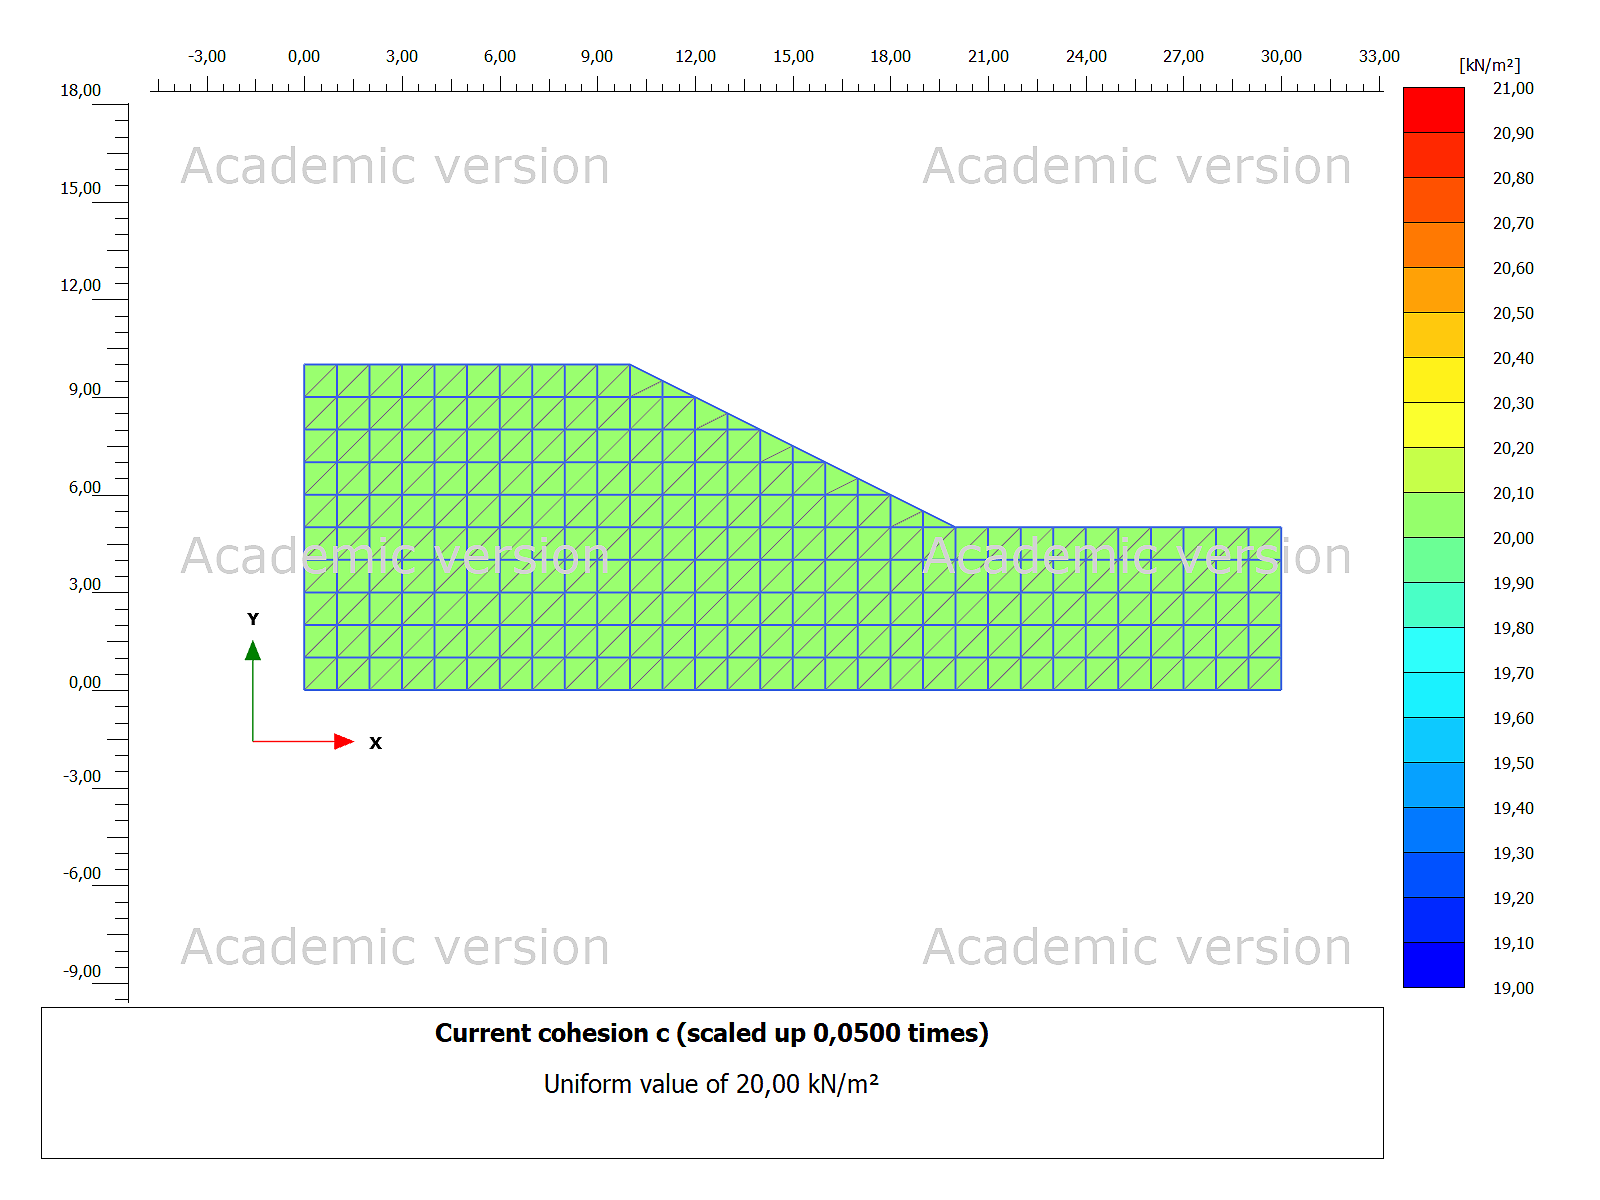
\includegraphics[width=\textwidth]{fig/testp}
	\caption{Slope geometry, with soil strength property from the random field mapped to the soil Plaxis soil elements and triangular FEM elements displayed}
	\label{fig:p2}
\end{figure}

\begin{figure}[h]
	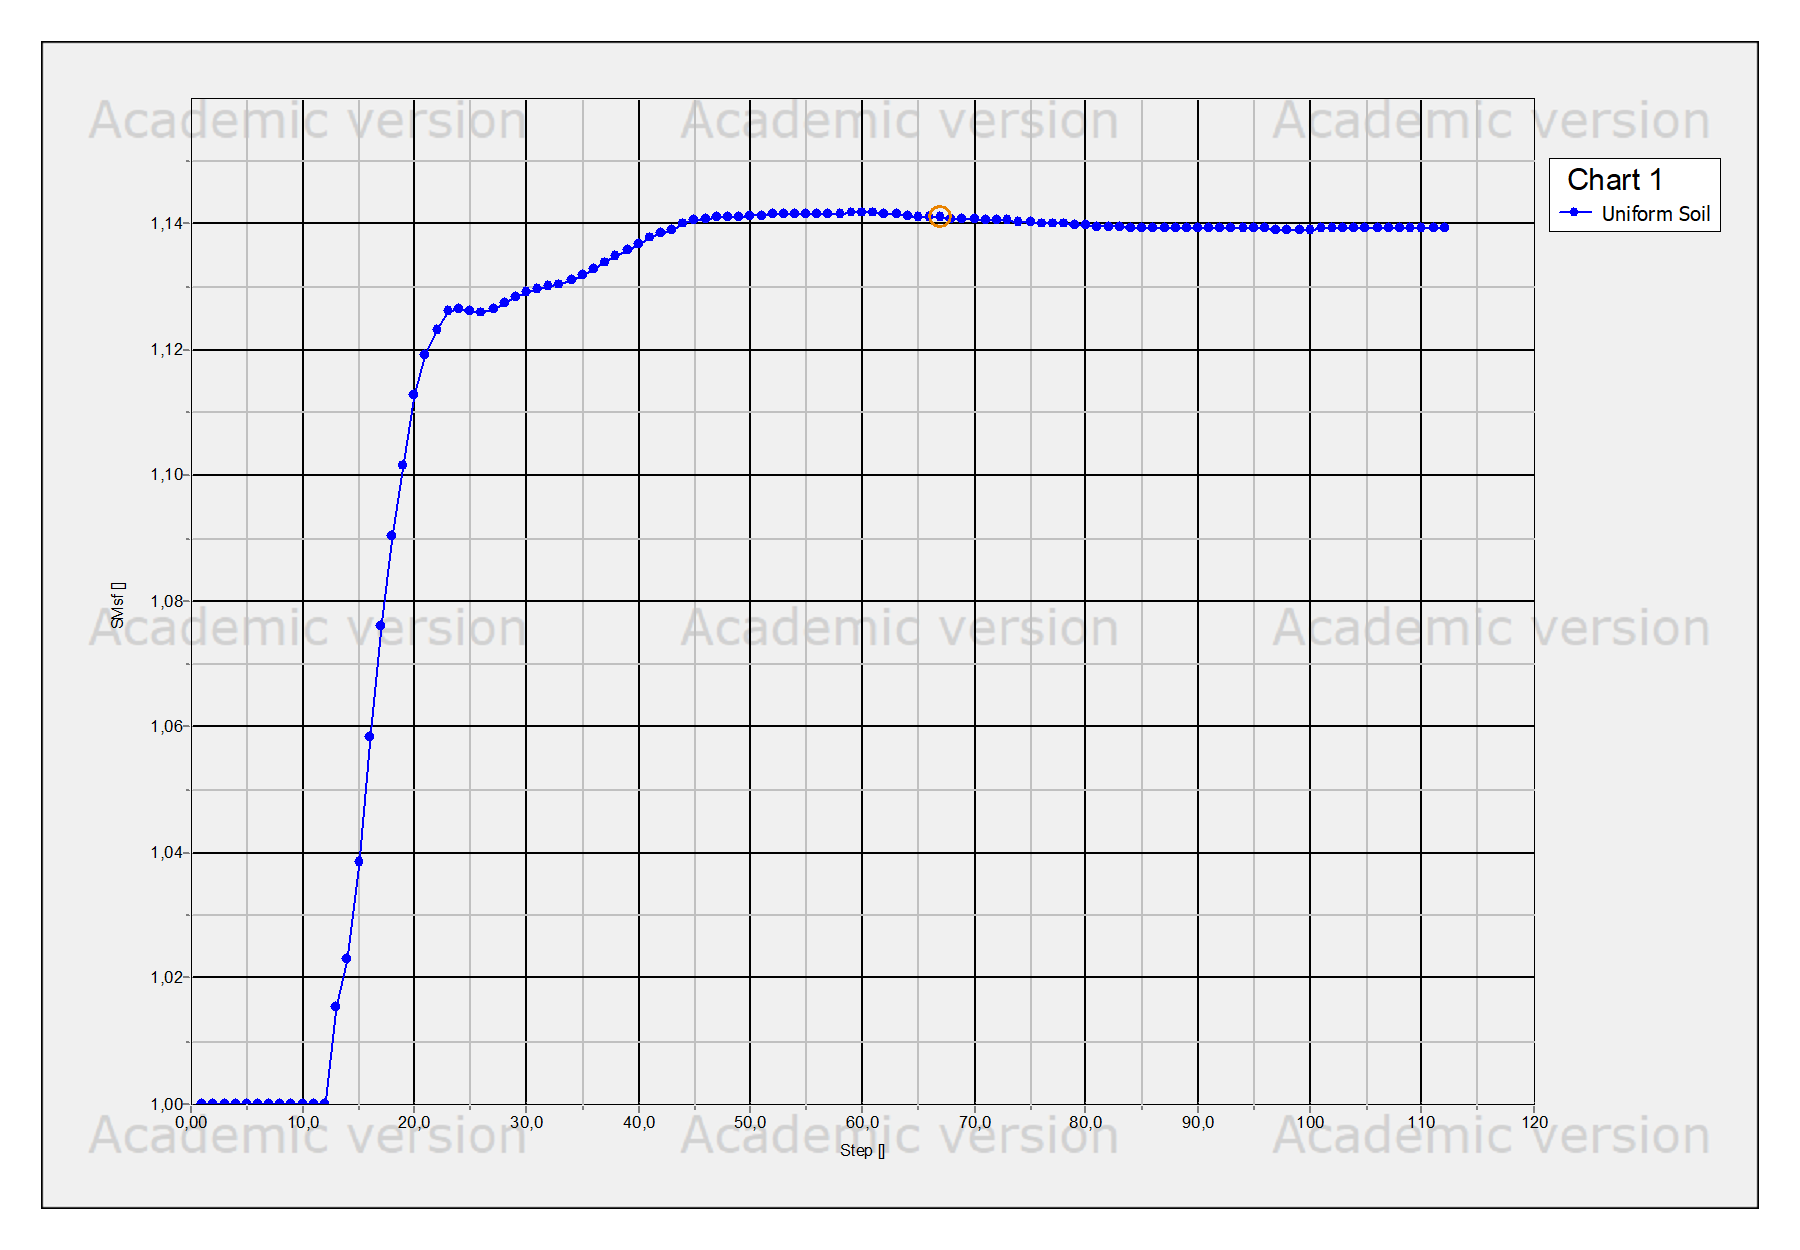
\includegraphics[width=\textwidth]{fig/Chart1}
	\caption{Plaxis Safety factor}
	\label{fig:psf1}
\end{figure}



\section{Slope stability problem - Homogeneous anisotropic soil - Scale of Fluctuation 20 and 10 meters, CoV=0.3 - Monte Carlo 250 realizations}


Following is the results from 250 realizations and simulations using random field as undrain strength parameters. The simulations are elasto-plastic FEM simulation with Mohr-Coulomb material model using Plaxis undraind(C) behaviour. 15-Node triangular FEM elements are used. The slope is 5 meter high with a 2:1 gradient.
The soil parameters is presented in Table \ref{tab2}. 
Examples of resulting random field is shown in \ref{fig:fourslopesfields}. 

Figure \ref{fig:mc4} shows the probability of failure of the slope vs iteration number. 

\begin{table}[h]
	\centering\small
	\caption{Soil parameters for anisotropic soil}
	\label{tab2}
		\begin{tabular*}{\textwidth}{@{\extracolsep{\fill}}lccc}
			\toprule
			 Soil model  &\multicolumn{3}{c}{Mohr Coulomb - Undrained(C)}\\
  \cmidrule{2-4}
			Statistical Soil	& Mean		 	& Coefficient of Variation 		& Scale of fluctuation \\
			Parameters	  	& $\mu$ 		&  $CoV = \frac{\sigma}{\mu}$ 		& $\theta_x$, $\theta_y$ \\
        
			\midrule
			  Unit weight, $\gamma_{sat}=\gamma{unsat}$ & 20 $kN/m^3$ & 0 & -,- \\
		          Modulus of elasticity, $E$ & 10 $MPa$ & 0 & - \\
		          Poissons ratio, $\nu$ & 0.49 & 0 & - \\
		          Undrained Shear Strength,$S_u$ & 20 $kPa$ & 0.3 & 20,10 \\
			\bottomrule
		\end{tabular*}
\end{table}


\begin{figure*}
\centering
\begin{subfigure}{0.475\textwidth}
    \centering
    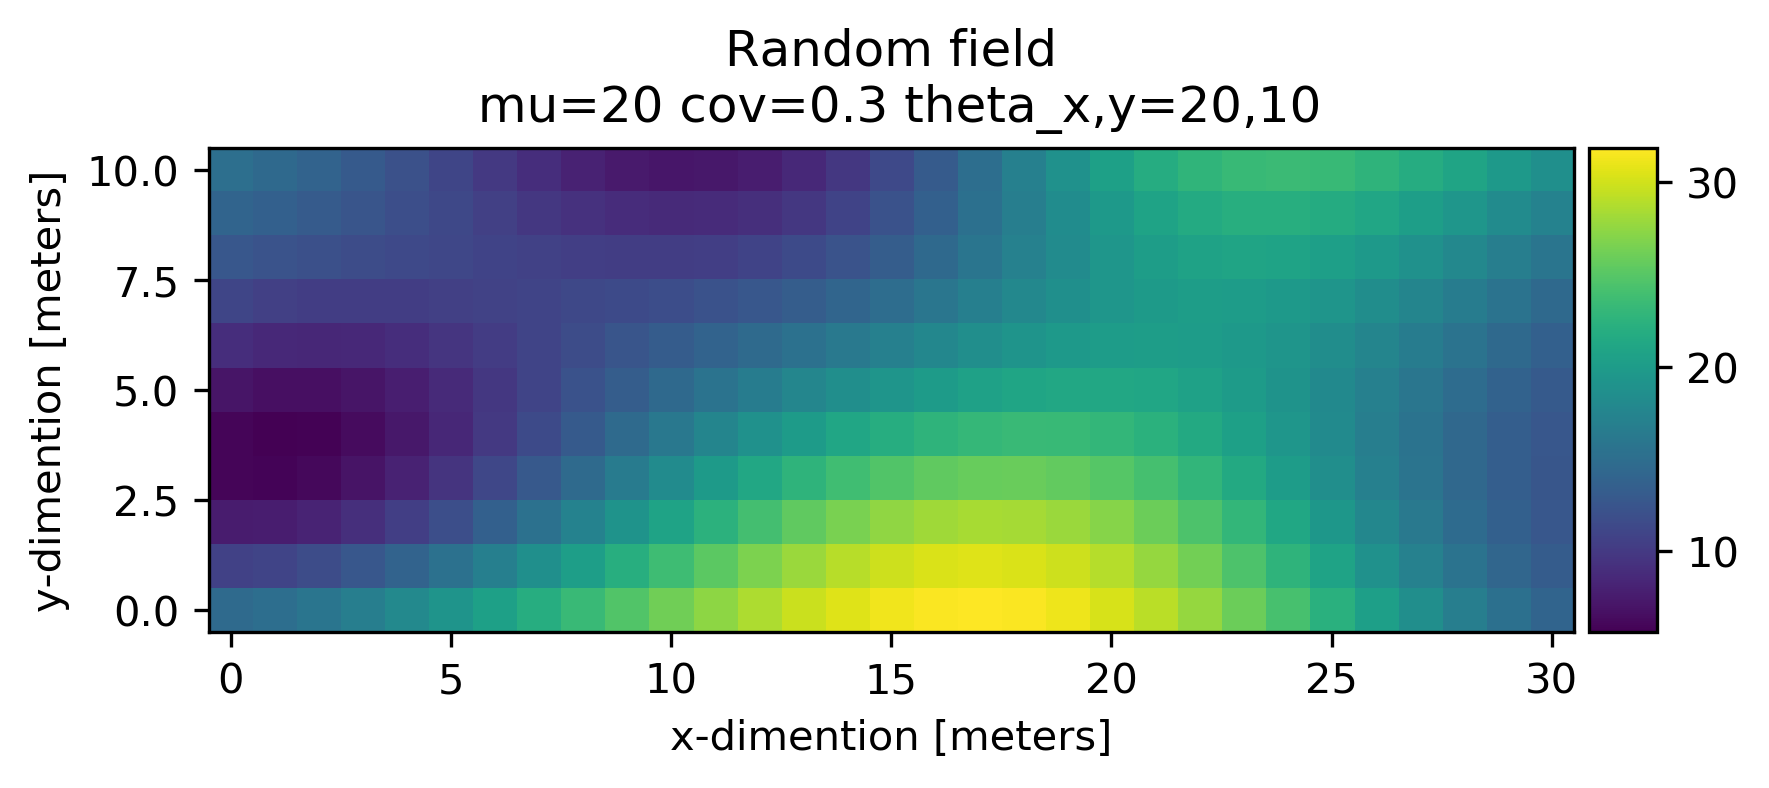
\includegraphics[width=\textwidth]{fig/ss/test20211118-125353}
    \caption[Network2]%
    {{\small Realization of undrained strength field, iteration 14 of 100}}
    \label{fig:mean and std of net14}
\end{subfigure}
\hfill
\begin{subfigure}{0.475\textwidth}
    \centering
    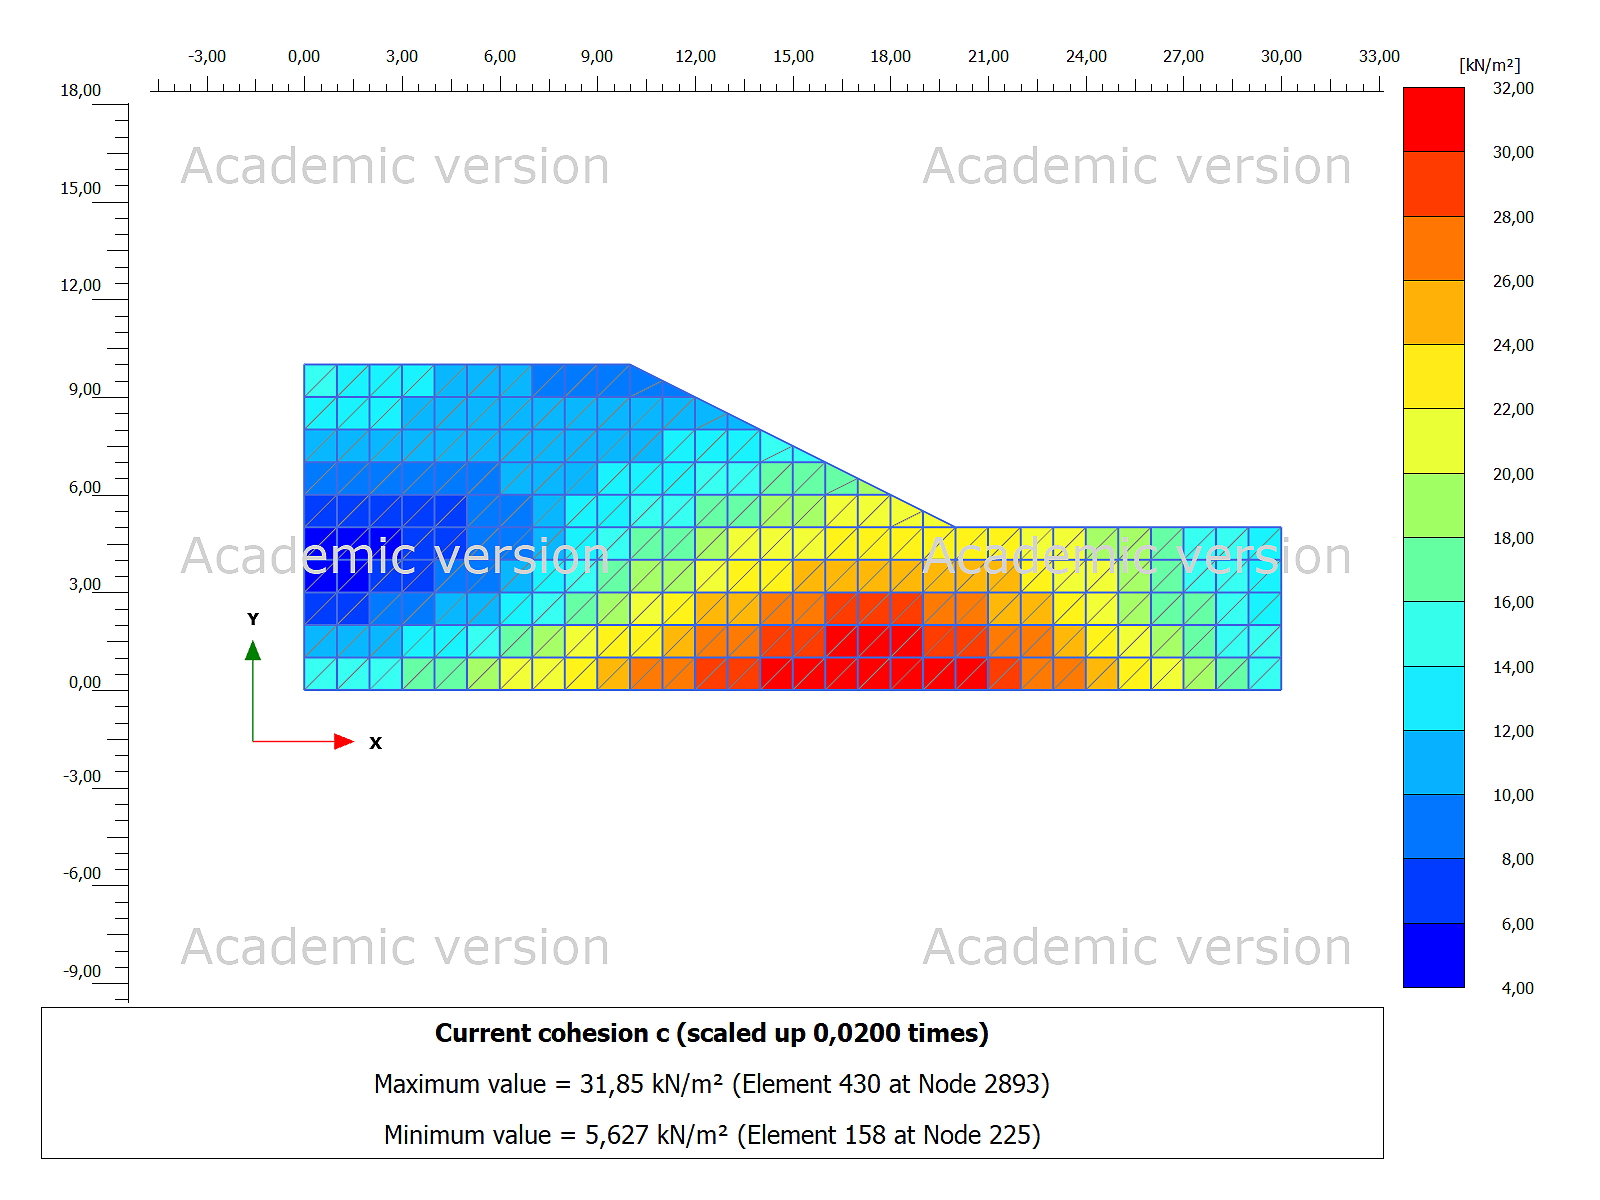
\includegraphics[width=\textwidth]{fig/ss/testp20211118-125455}
    \caption[]%
    {{\small Realization of undrained strength field, iteration 45 of 100}}
    \label{fig:mean and std of net24}
\end{subfigure}
\vskip\baselineskip
\begin{subfigure}{0.475\textwidth}
    \centering
    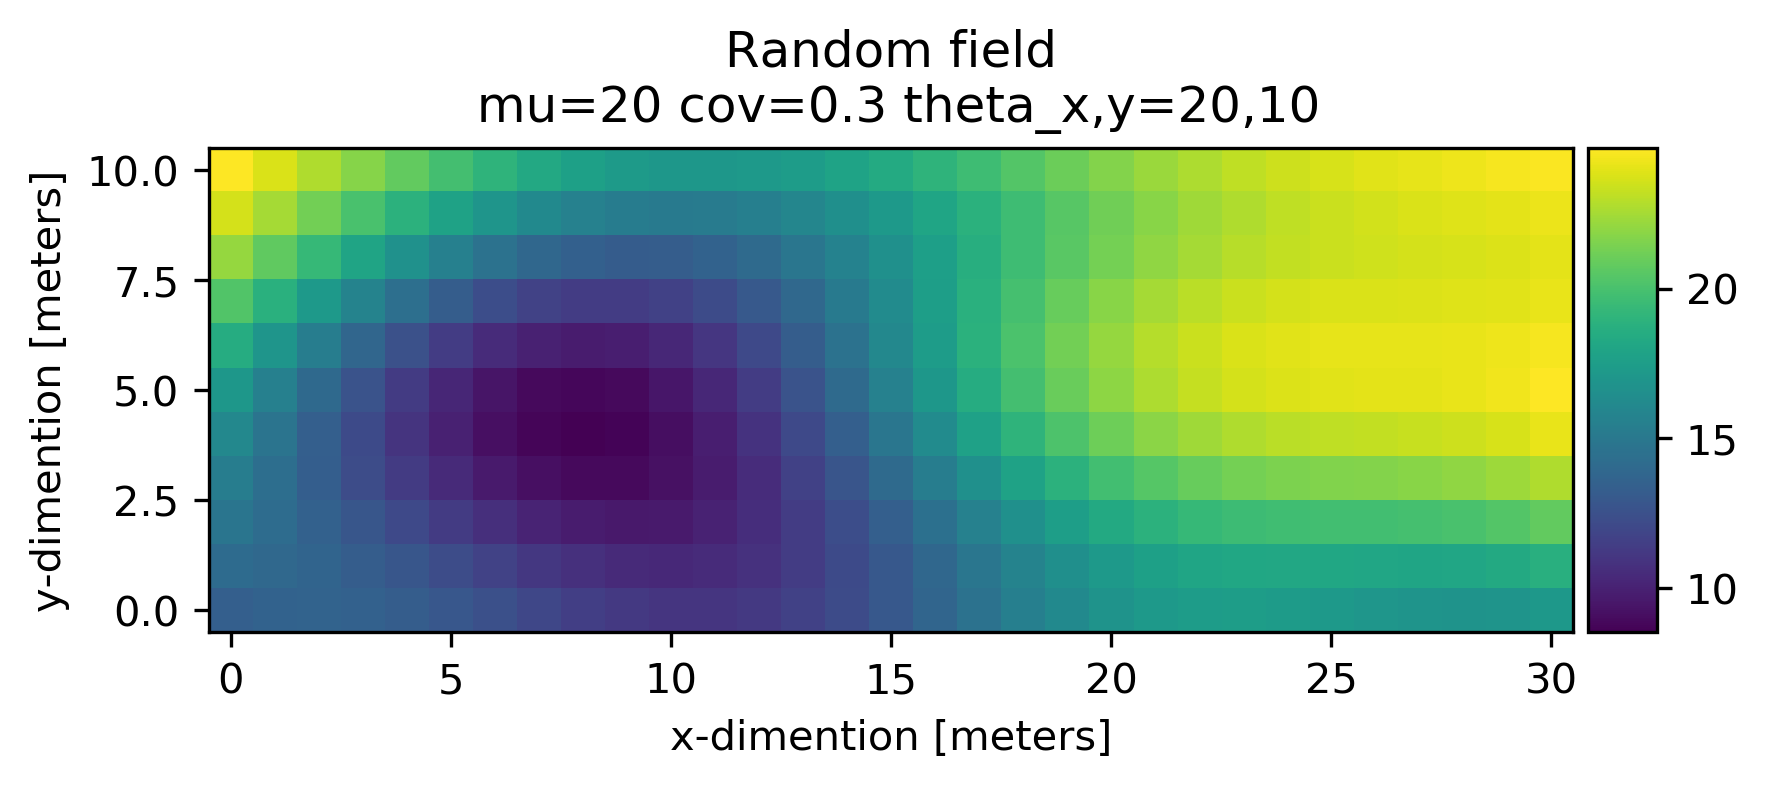
\includegraphics[width=\textwidth]{fig/ss/test20211118-125713}
    \caption[]%
    {{\small Realization of undrained strength field, iteration 70 of 100}}
    \label{fig:mean and std of net34}
\end{subfigure}
\hfill
\begin{subfigure}{0.475\textwidth}
    \centering
    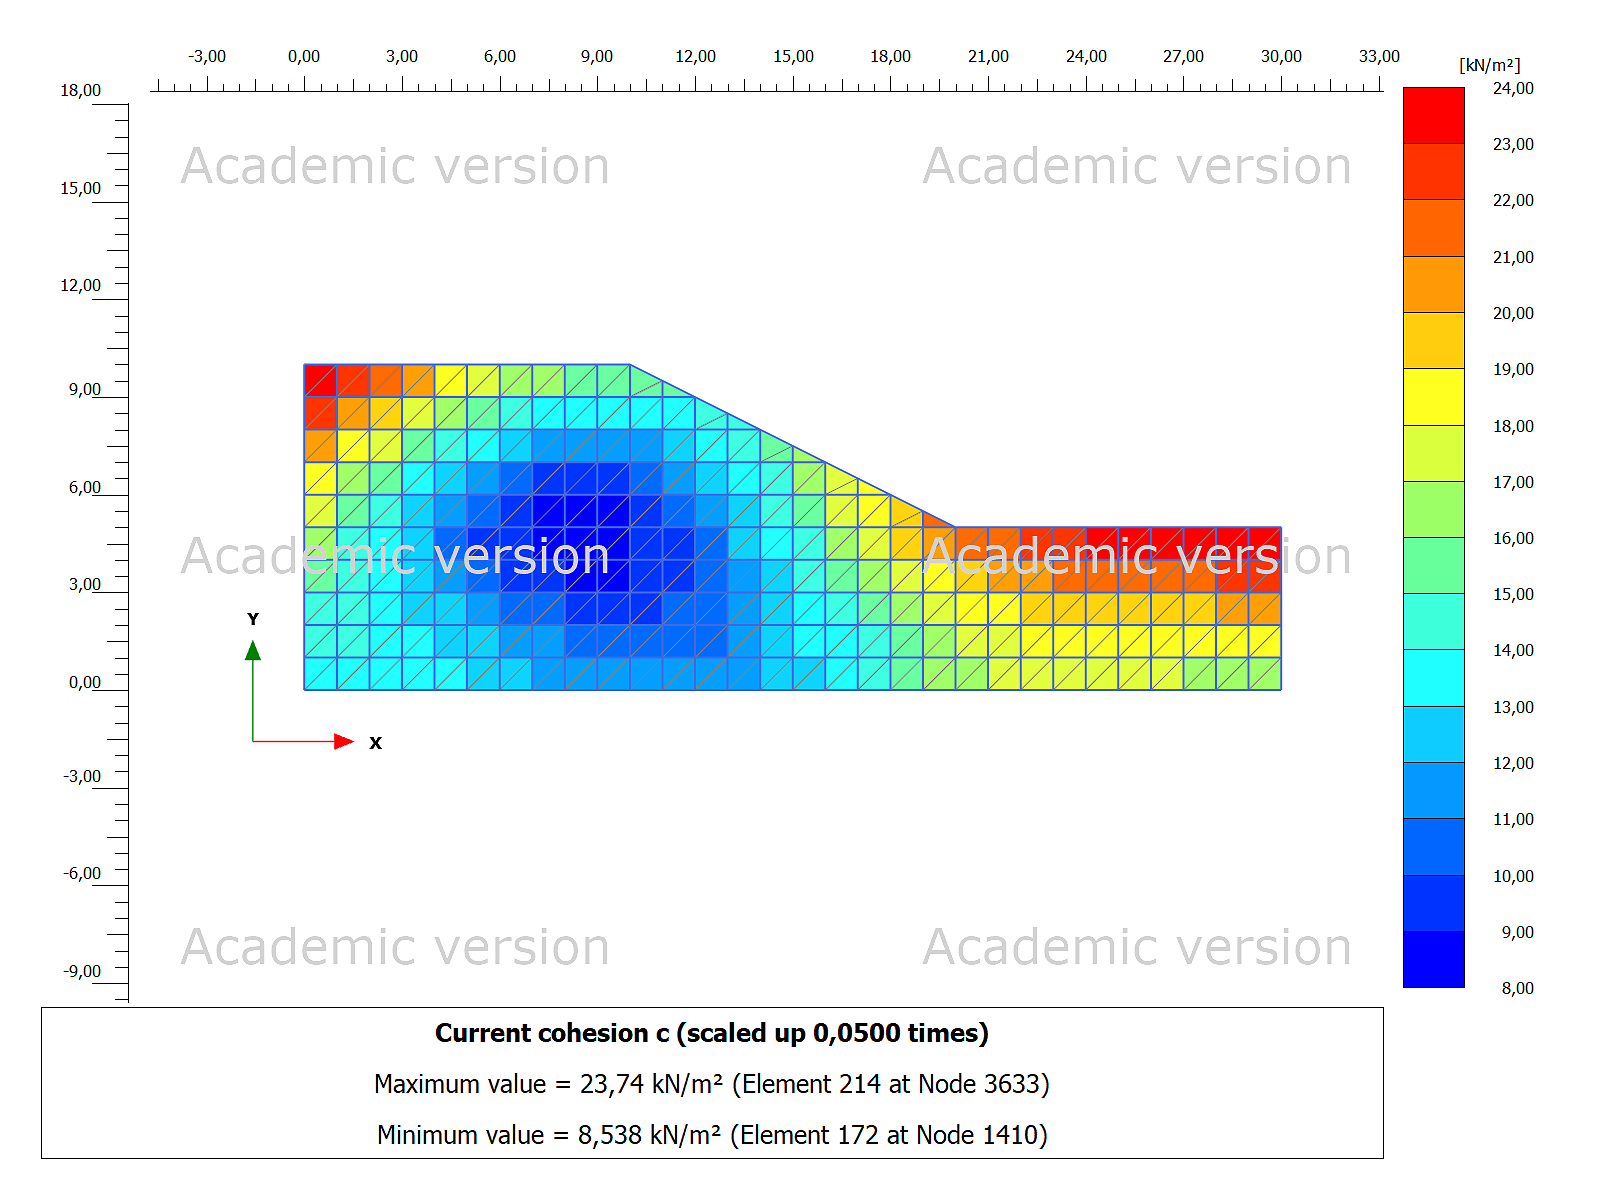
\includegraphics[width=\textwidth]{fig/ss/testp20211118-125818}
    \caption[]%
    {{\small Realization of undrained strength field, iteration 81 of 100}}
    \label{fig:mean and std of net44}
\end{subfigure}
\begin{subfigure}{0.475\textwidth}
    \centering
    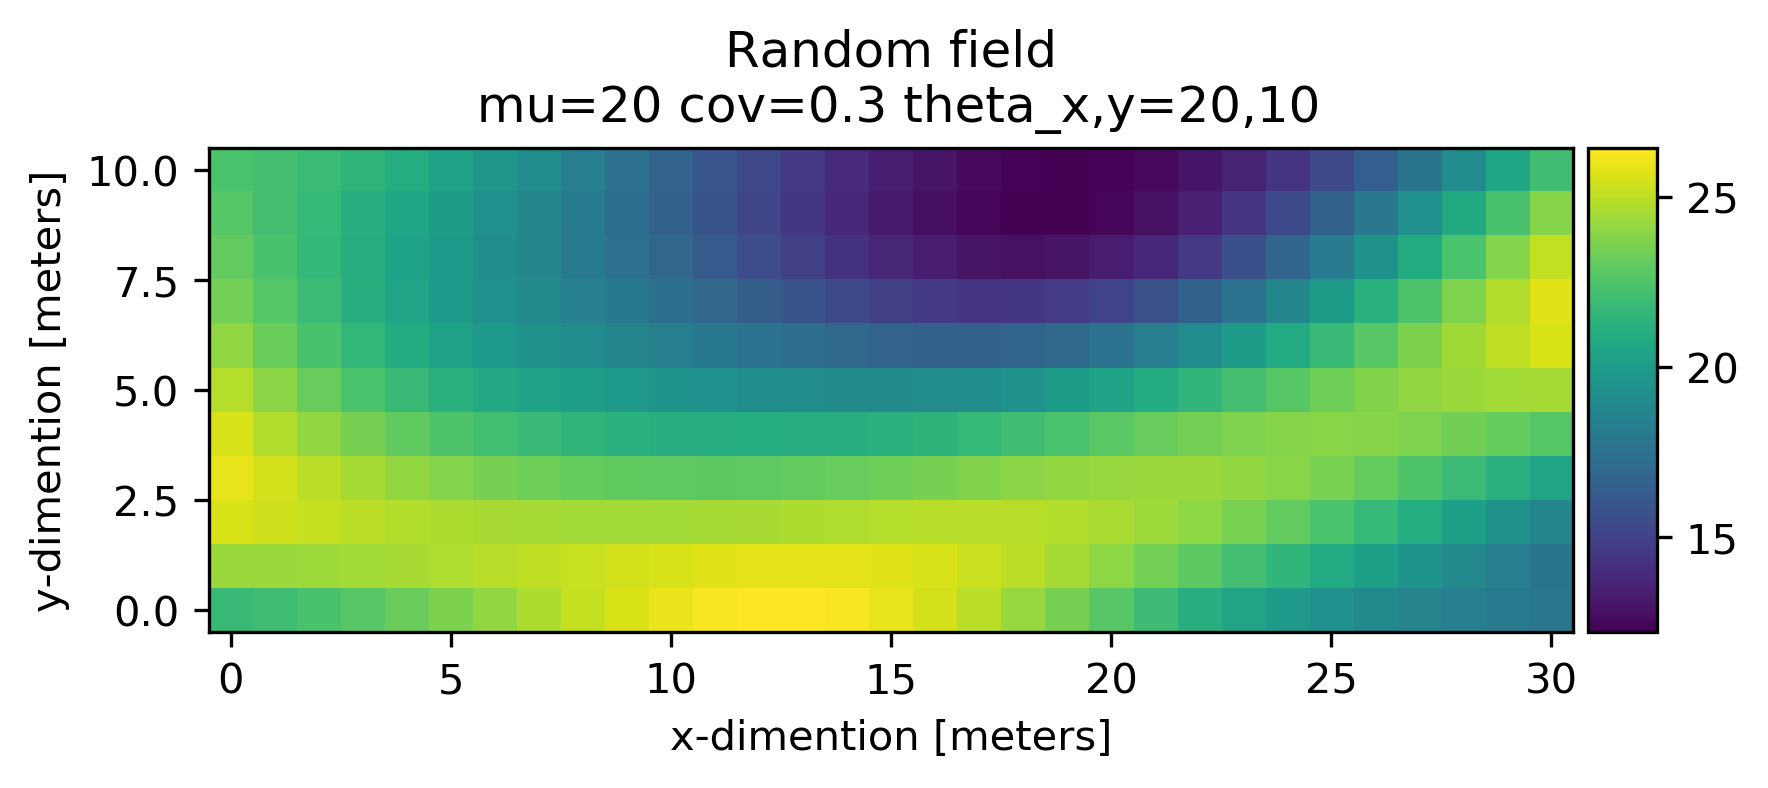
\includegraphics[width=\textwidth]{fig/ss/test20211118-125941}
    \caption[]%
    {{\small Realization of undrained strength field, iteration 70 of 100}}
    \label{fig:mean and std of net56}
\end{subfigure}
\hfill
\begin{subfigure}{0.475\textwidth}
    \centering
    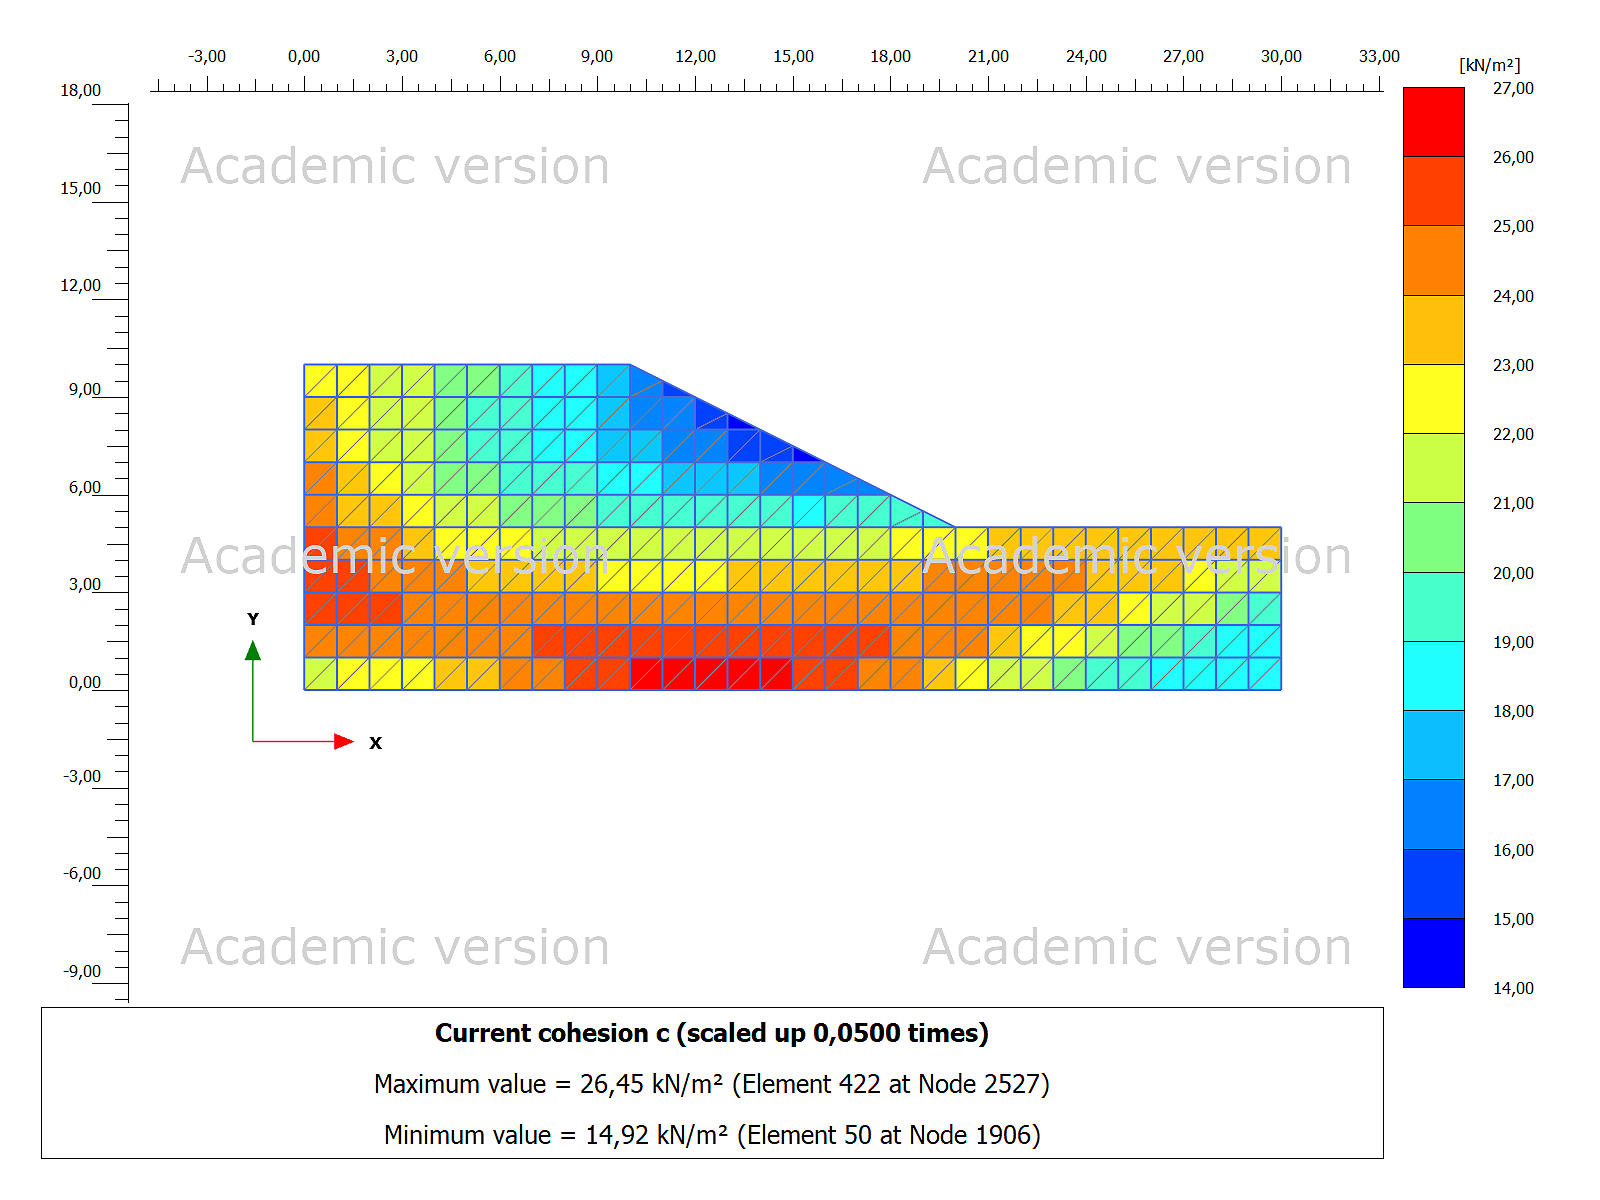
\includegraphics[width=\textwidth]{fig/ss/testp20211118-130042}
    \caption[]%
    {{\small Realization of undrained strength field, iteration 81 of 100}}
    \label{fig:mean and std of net66}
\end{subfigure}
\caption[ Three different realizations of random fields created by SRM.]
{\small Three different realizations of random fields created by SRM.}
\label{fig:fourslopesfields}
\end{figure*}


\begin{figure}[h]
	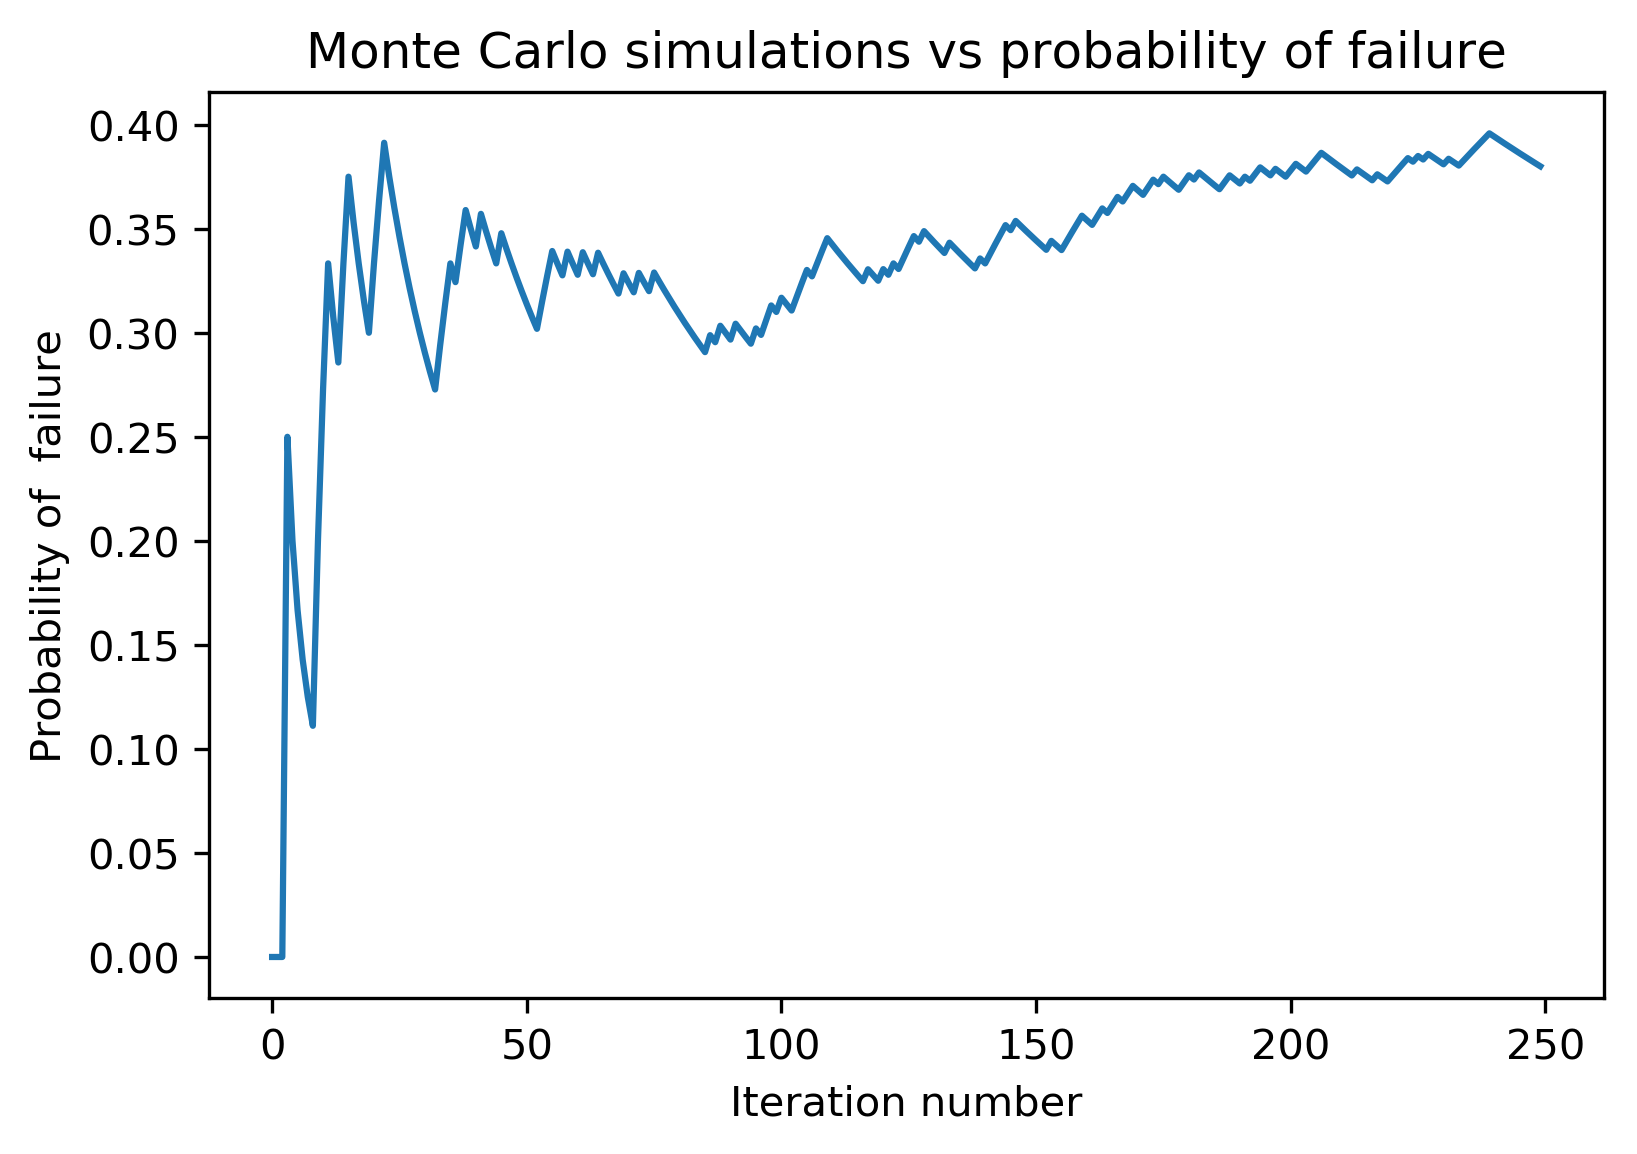
\includegraphics[width=\textwidth]{fig/pfailit20211116-090042}
	\caption{Iteration number vs probability of failure for the Monte Carlo RFEM slope stability problem. The failure probability converges towards a value of around 0.38. More iterations might be needed to see if the result is stable.}
	\label{fig:mc4}
\end{figure}

\section{Bearing Capacity Problem - Homogeneous isotropic soil - CoV=0.0 - Known analytical solution}

To illustrate the versatility of the implementation, the slope stability problem is changed to a bearing capacity problem by specifying a flat topology and adding a line load.
This change is done wit the change of 2 lines of code.
To verify the validity, again a base case with an analytical solution is set up. Undrained bearing capacity for a smooth foundation with the known bearing capacity:
\begin{equation}
	\label{eq:bc_su}
	q = 5.14 S_u 
\end{equation}
The simulation is a elasto-plastic FEM simulation with Mohr-Coulomb material model using Plaxis undraind(C) behaviour. 15-Node triangular FEM elements are used. A line load of 1000kPa and length of 9 meters is applied to the top of the soil. 
The soil parameters is presented in Table \ref{tab:bc_su}. 
Internal in the Plaxis code, ref step 6 in chapter 3.3, the 1000 kPa load is applied in increments, the fraction of the load applied is given in in the Plaxis variable called $\sum M stage$. see Figure \ref{fig:bc_su4} for simulation result.
The bearing capacity of the soil is given as:
\begin{equation}
	\label{eq:bc_su2}
	q = 1000*\sum M Stage = 1000 * 0.103 = 103 
\end{equation}

Equation \ref{eq:bc_su} gives for $S_u = 20$ , $q=5.14 S_u = 5.14 * 20 = 102.8$. The result of the simulation gives a good approximation. 

The soil field, in this particular case a constant field, is shown in Figure \ref{fig:bc_su1} and bearing capacity geometry, load and Plaxis 2D mesh is shown in Figure \ref{fig:bc_su2}. The failure mechanism is illustrated in \ref{fig:bc_su3}


\begin{table}[h]
	\centering\small
	\caption{Soil parameters for anisotropic soil}
	\label{tab:bc_su}
		\begin{tabular*}{\textwidth}{@{\extracolsep{\fill}}lccc}
			\toprule
			 Soil model  &\multicolumn{3}{c}{Mohr Coulomb - Undrained(C)}\\
  \cmidrule{2-4}
			Statistical Soil	& Mean		 	& Coefficient of Variation 		& Scale of fluctuation \\
			Parameters	  	& $\mu$ 		&  $CoV = \frac{\sigma}{\mu}$ 		& $\theta_x$ and $\theta_y$ \\
        
			\midrule
			  Unit weight, $\gamma_{sat}=\gamma{unsat}$ & 20 $kN/m^3$ & 0 & -,- \\
		          Modulus of elasticity, $E$ & 10 $MPa$ & 0 & - \\
		          Poissons ratio, $\nu$ & 0.49 & 0 & - \\
		          Undrained Shear Strength,$S_u$ & 20 $kPa$ & 0 & 0 and 0 \\
			\bottomrule
		\end{tabular*}
\end{table}

\begin{figure}[h]
	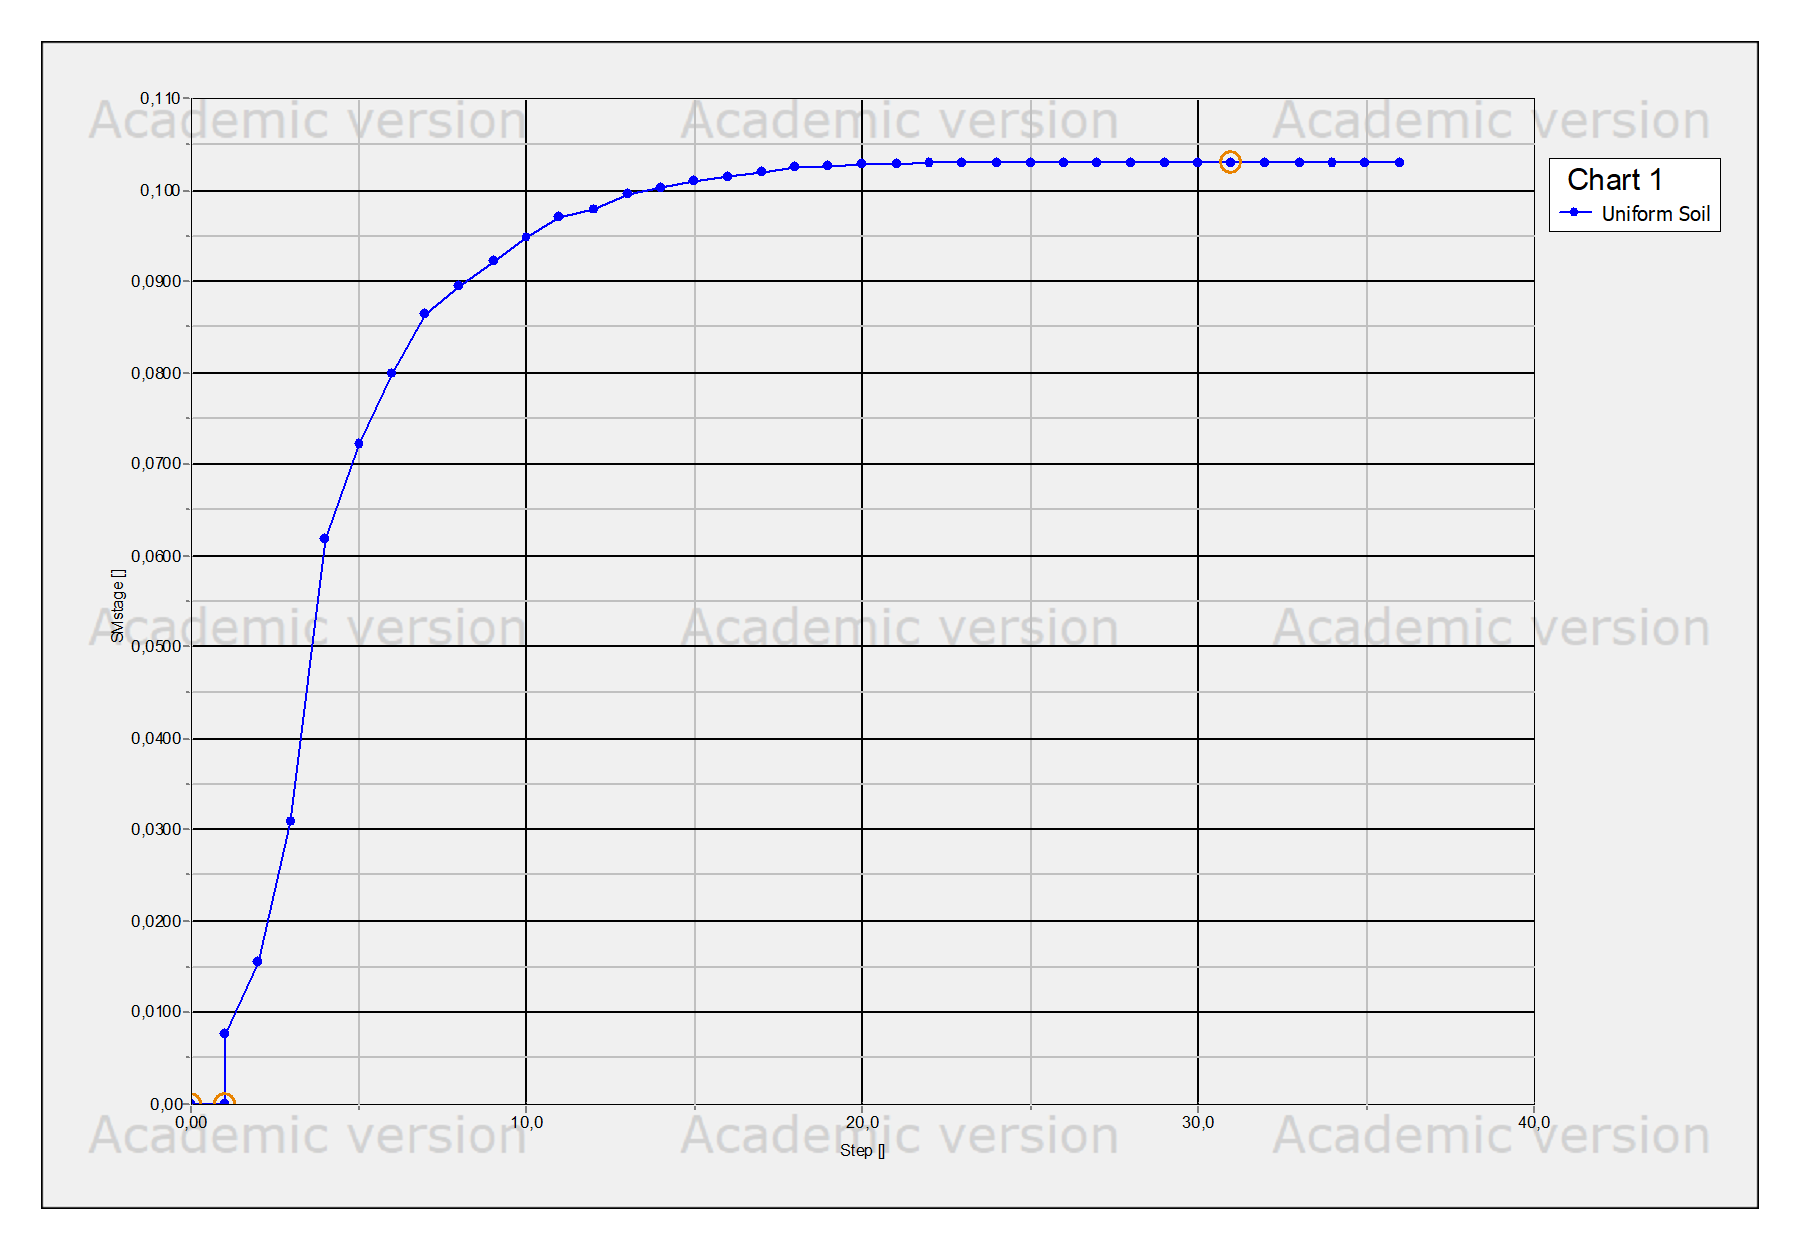
\includegraphics[width=\textwidth]{fig/bc/Chart2}
	\caption{Bearing Capacity problem for uniform soil. Plaxis 2D Load step vs fraction of applied load. Failure occur at 0.103 times the applied load of 1000 kPa}
	\label{fig:bc_su4}
\end{figure}
\begin{figure}[h]
	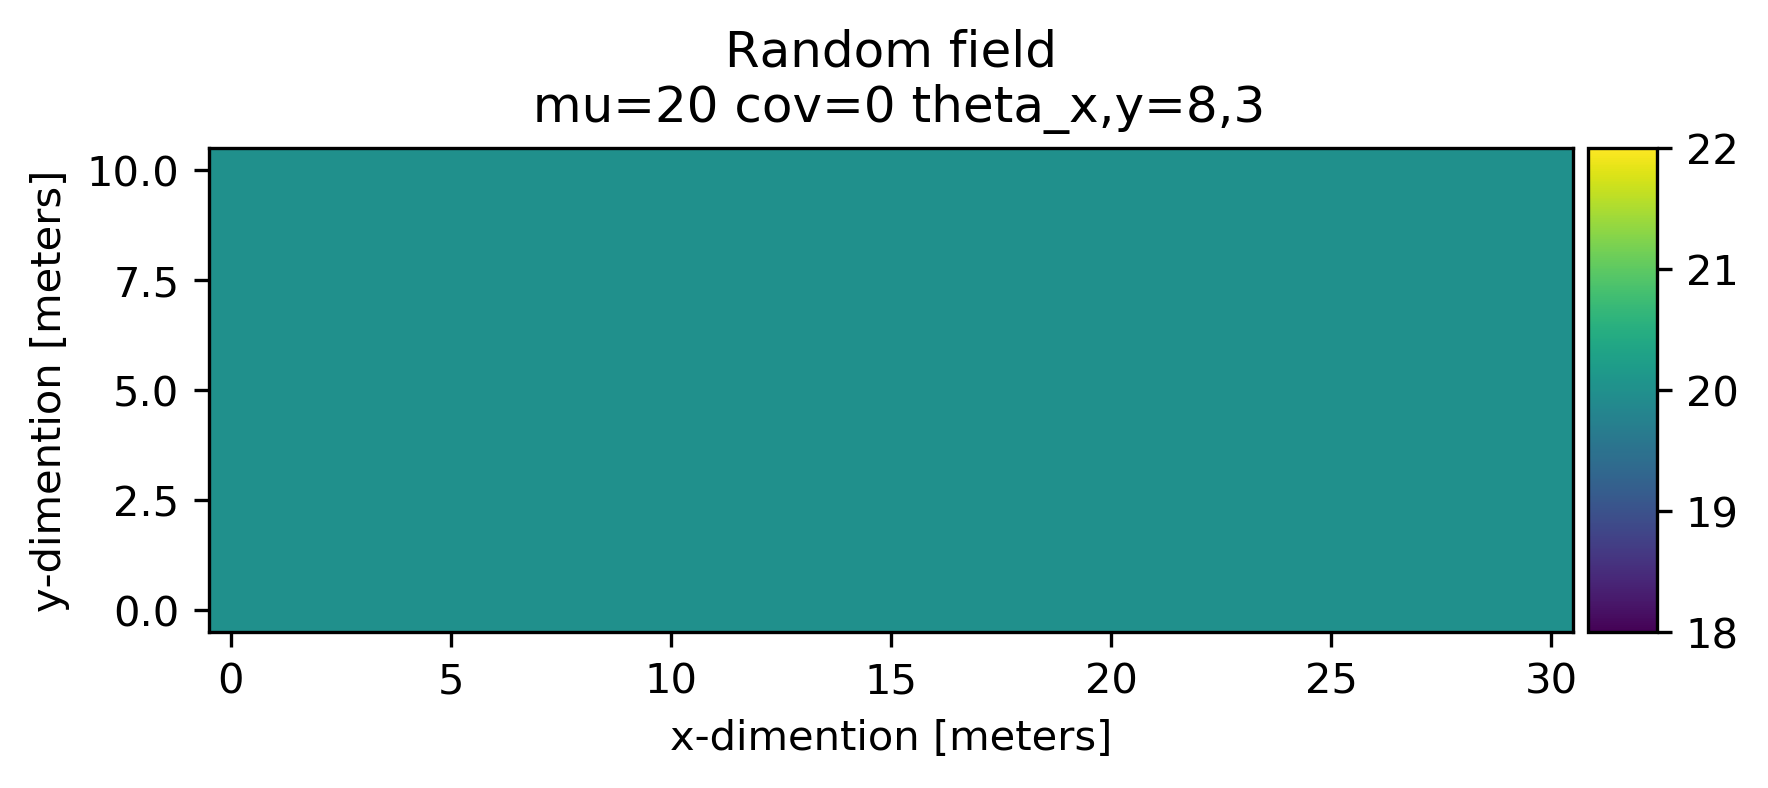
\includegraphics[width=\textwidth]{fig/bc/test20211116-100048}
	\caption{Uniform undrained soil shear strength of 20 kPa used in bearing capacity verification simulation}
	\label{fig:bc_su1}
\end{figure}
\begin{figure}[h]
	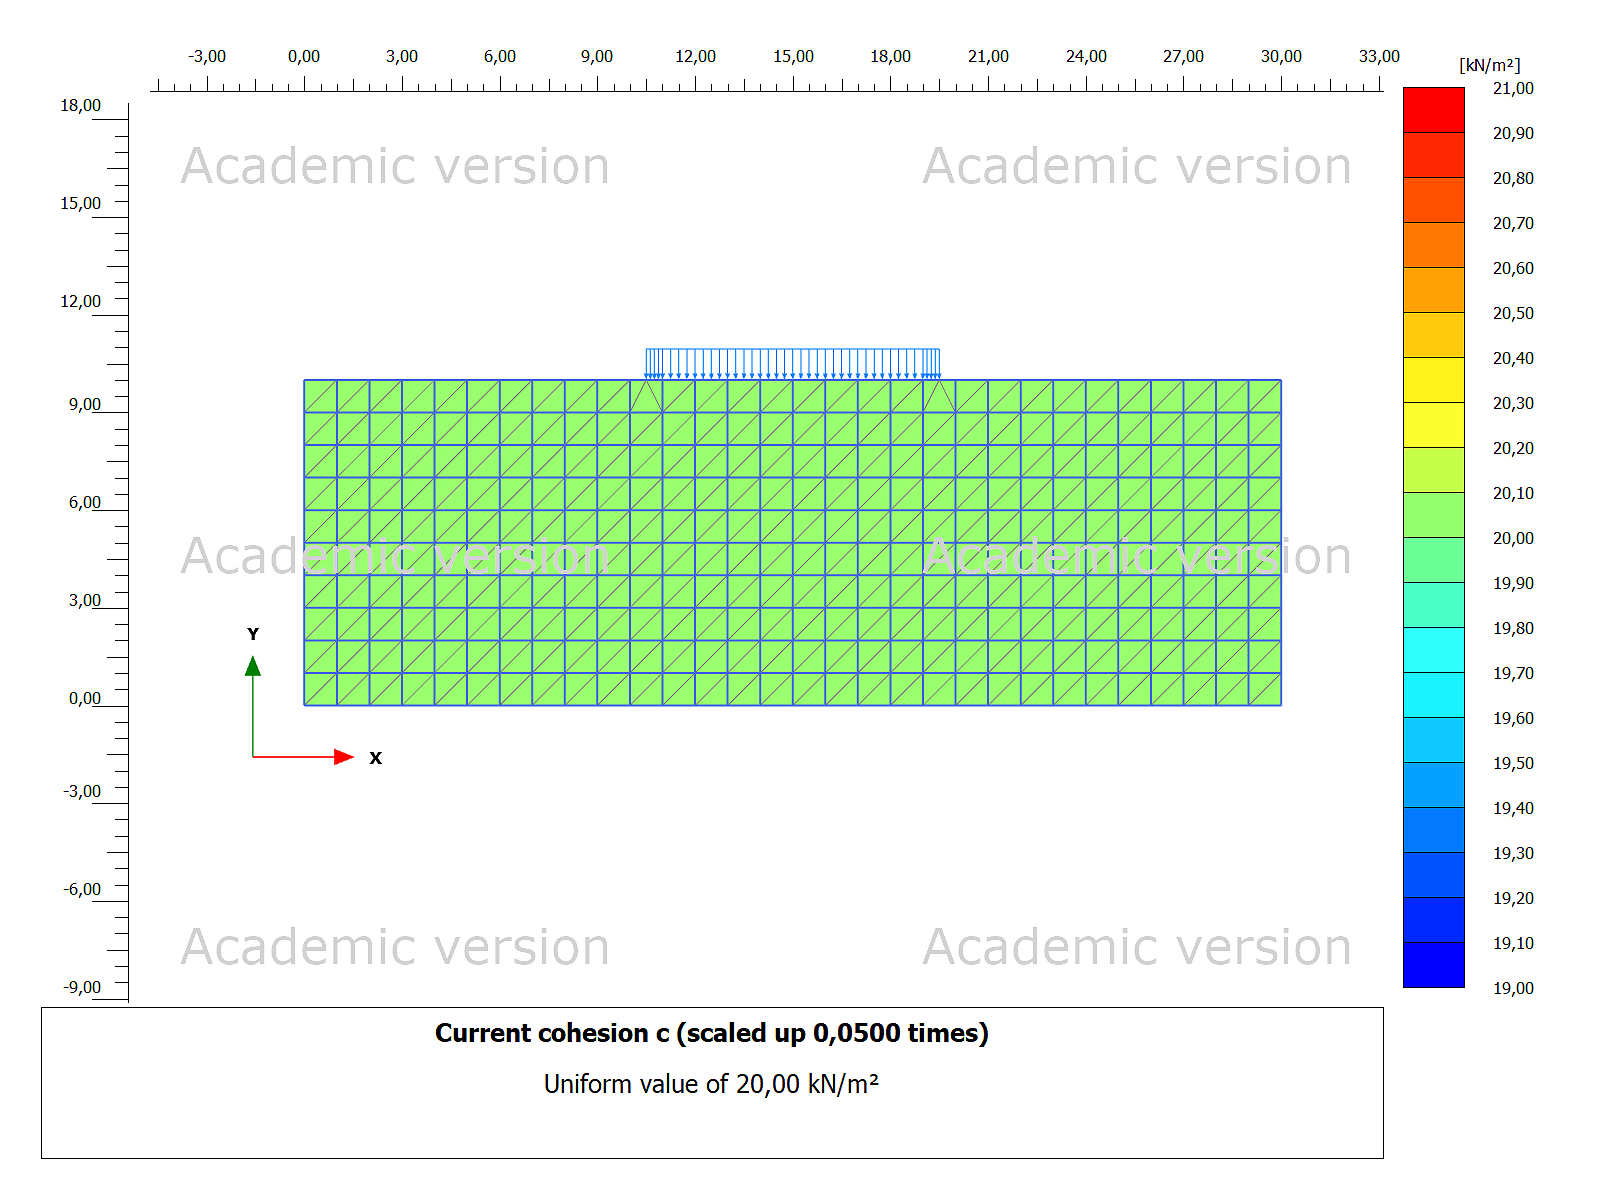
\includegraphics[width=\textwidth]{fig/bc/testp20211116-100145}
	\caption{Bearing capacity problem geometry, load and FEM mesh.}
	\label{fig:bc_su2}
\end{figure}
\begin{figure}[h]
	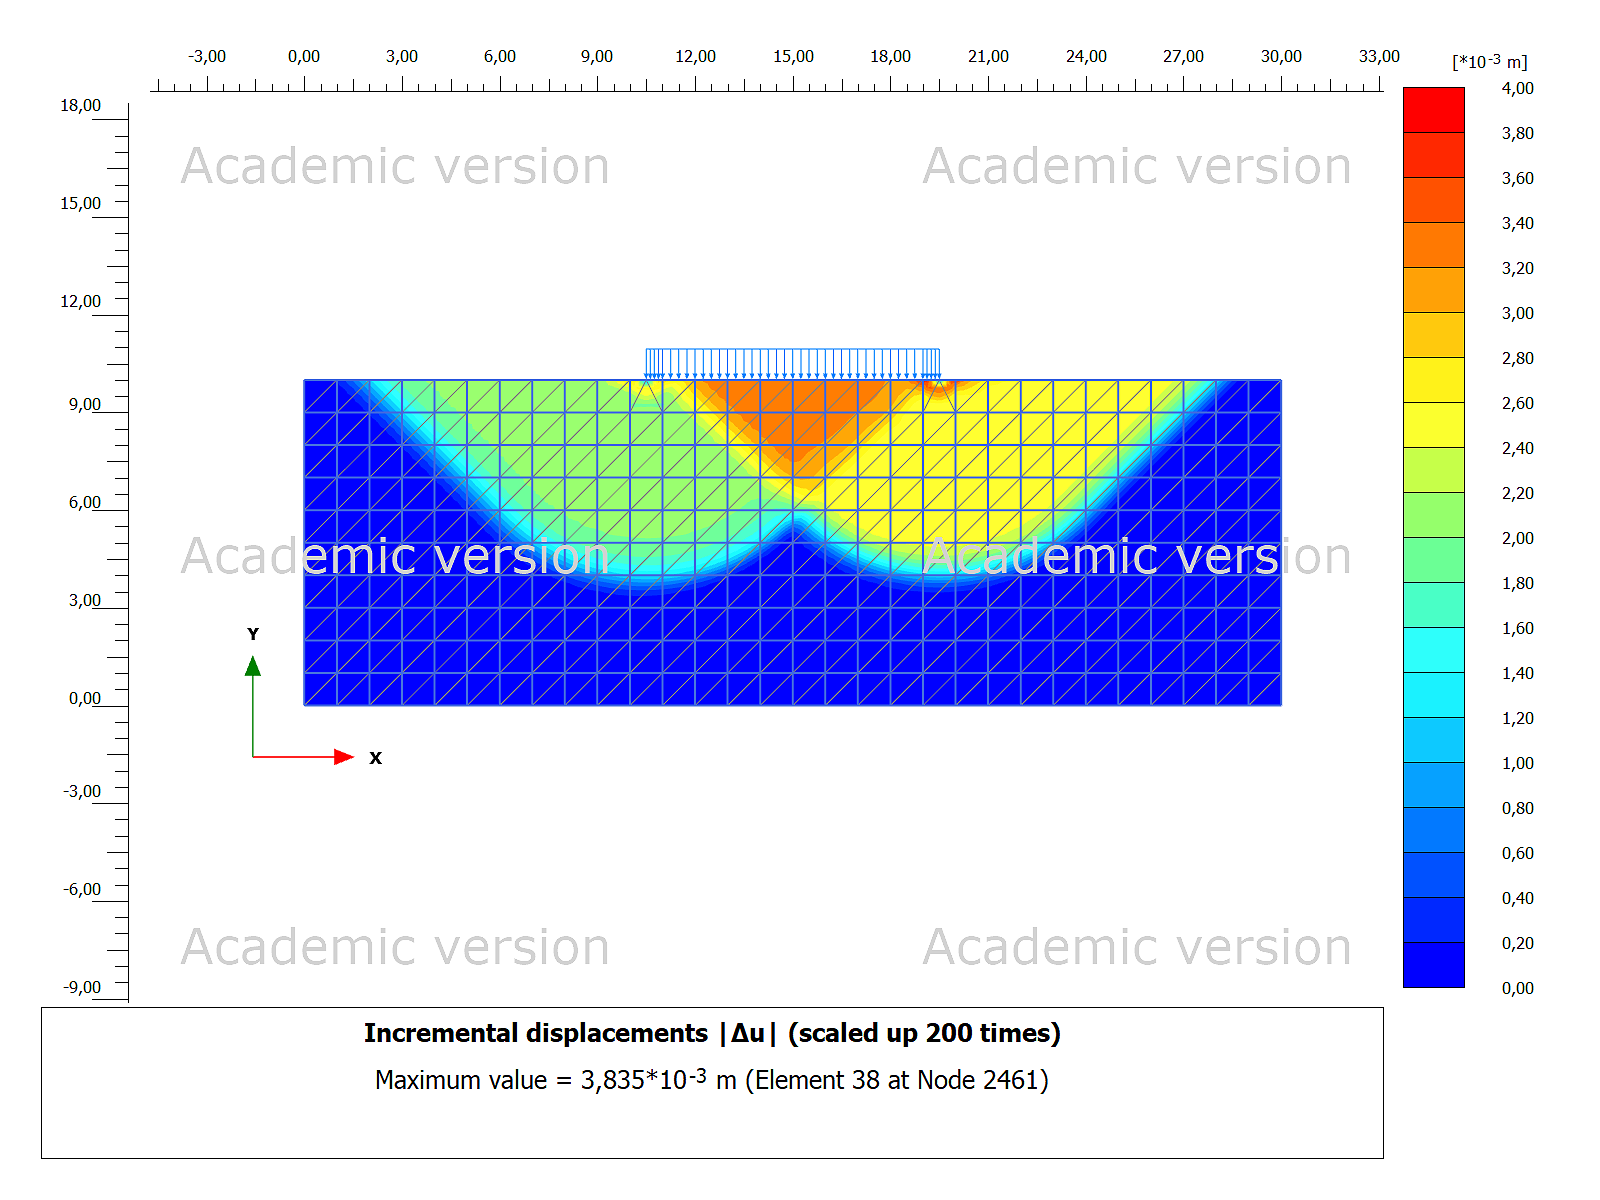
\includegraphics[width=\textwidth]{fig/bc/testutot20211116-100146}
	\caption{Illustration of failure mechanism for the bearing capacity verification simulation}
	\label{fig:bc_su3}
\end{figure}

\section{Bearing Capacity Problem - Homogeneous anisotropic soil - Scale of Fluctuation 8 and 3 meters, CoV=0.1, Monte Carlo 250 realizations}
The bearing capacity problem is repeated with a random field input representing the soil undrained strength.The soil parameters are given in table \ref{tab:bc_su2}. 
250 iterations are run in a Monte Carlo simulation. The FEM parametrisation is the same as for the other problems, repeated here: 
Elasto-plastic FEM simulation with Mohr-Coulomb material model using Plaxis undraind(C) behaviour. 15-Node triangular FEM elements are used.
\begin{table}[h]
	\centering\small
	\caption{Soil parameters for anisotropic soil}
	\label{tab:bc_su2}
		\begin{tabular*}{\textwidth}{@{\extracolsep{\fill}}lccc}
			\toprule
			 Soil model  &\multicolumn{3}{c}{Mohr Coulomb - Undrained(C)}\\
  \cmidrule{2-4}
			Statistical Soil	& Mean		 	& Coefficient of Variation 		& Scale of fluctuation \\
			Parameters	  	& $\mu$ 		&  $CoV = \frac{\sigma}{\mu}$ 		& $\theta_x$, $\theta_y$ \\
        
			\midrule
			  Unit weight, $\gamma_{sat}=\gamma{unsat}$ & 20 $kN/m^3$ & 0 & -,- \\
		          Modulus of elasticity, $E$ & 10 $MPa$ & 0 & - \\
		          Poissons ratio, $\nu$ & 0.49 & 0 & - \\
		          Undrained Shear Strength,$S_u$ & 20 $kPa$ & 0.3 & 8,3 \\
			\bottomrule
		\end{tabular*}
\end{table}

The resulting bearing capacities from the 250 realizations of the random finite element run is displayed in a histogram in Figure \ref{fig:bc_hist}. Note that all bearing capacities is lower than that for uniform soil with constant undrained shear strength equal to the mean $S_u$ in the RFEM run.

Figure \ref{fig:sixbcfields} shows three random realizations from the RFEM run and the corresponding variety in failure mechanism. 

\begin{figure}[h]
	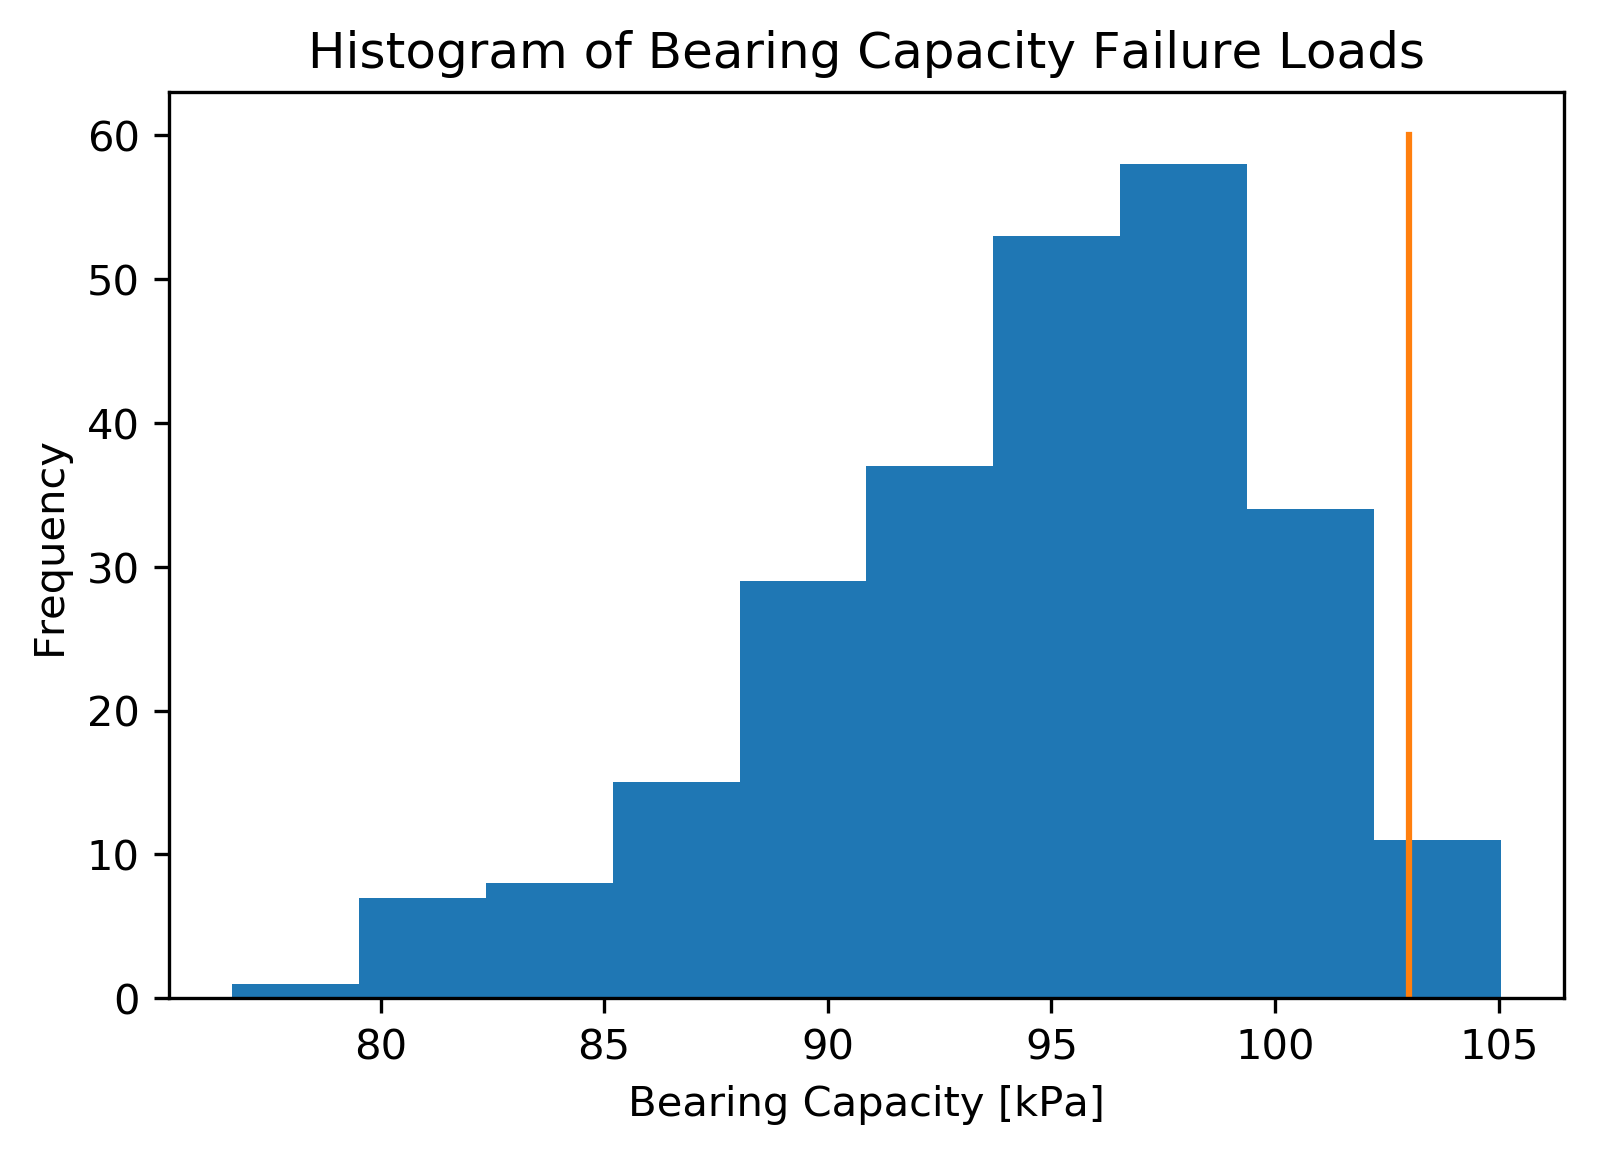
\includegraphics[width=\textwidth]{fig/bc/nx/bc_histogram20211117-091648}
	\caption{Histogram of Bering Capacities from 250 iterations of RFEM}
	\label{fig:bc_hist}
\end{figure}


\begin{figure*}
\centering
\begin{subfigure}{0.475\textwidth}
    \centering
    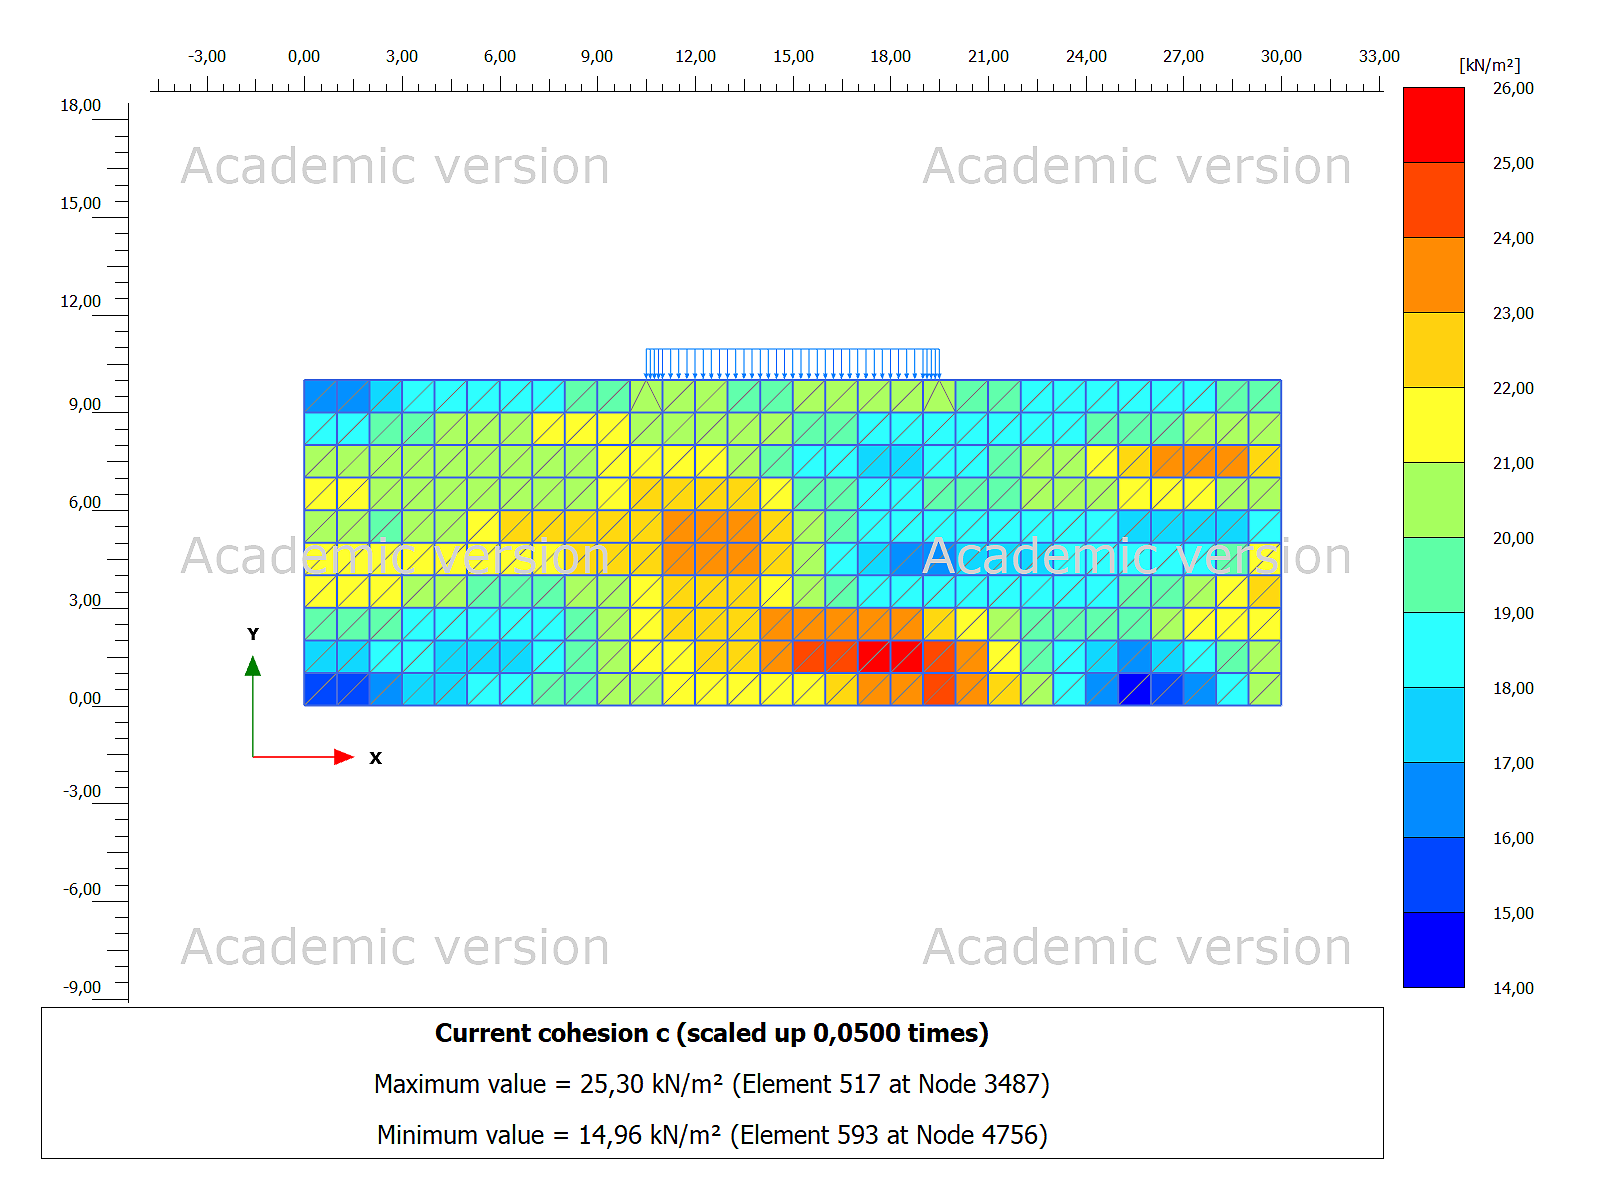
\includegraphics[width=\textwidth]{fig/bc/nx/testp20211116-101822}
    \caption[Network2]%
    {{\small Realization of undrained strength field, iteration 201}}
    \label{fig:bc net14}
\end{subfigure}
\hfill
\begin{subfigure}{0.475\textwidth}
    \centering
    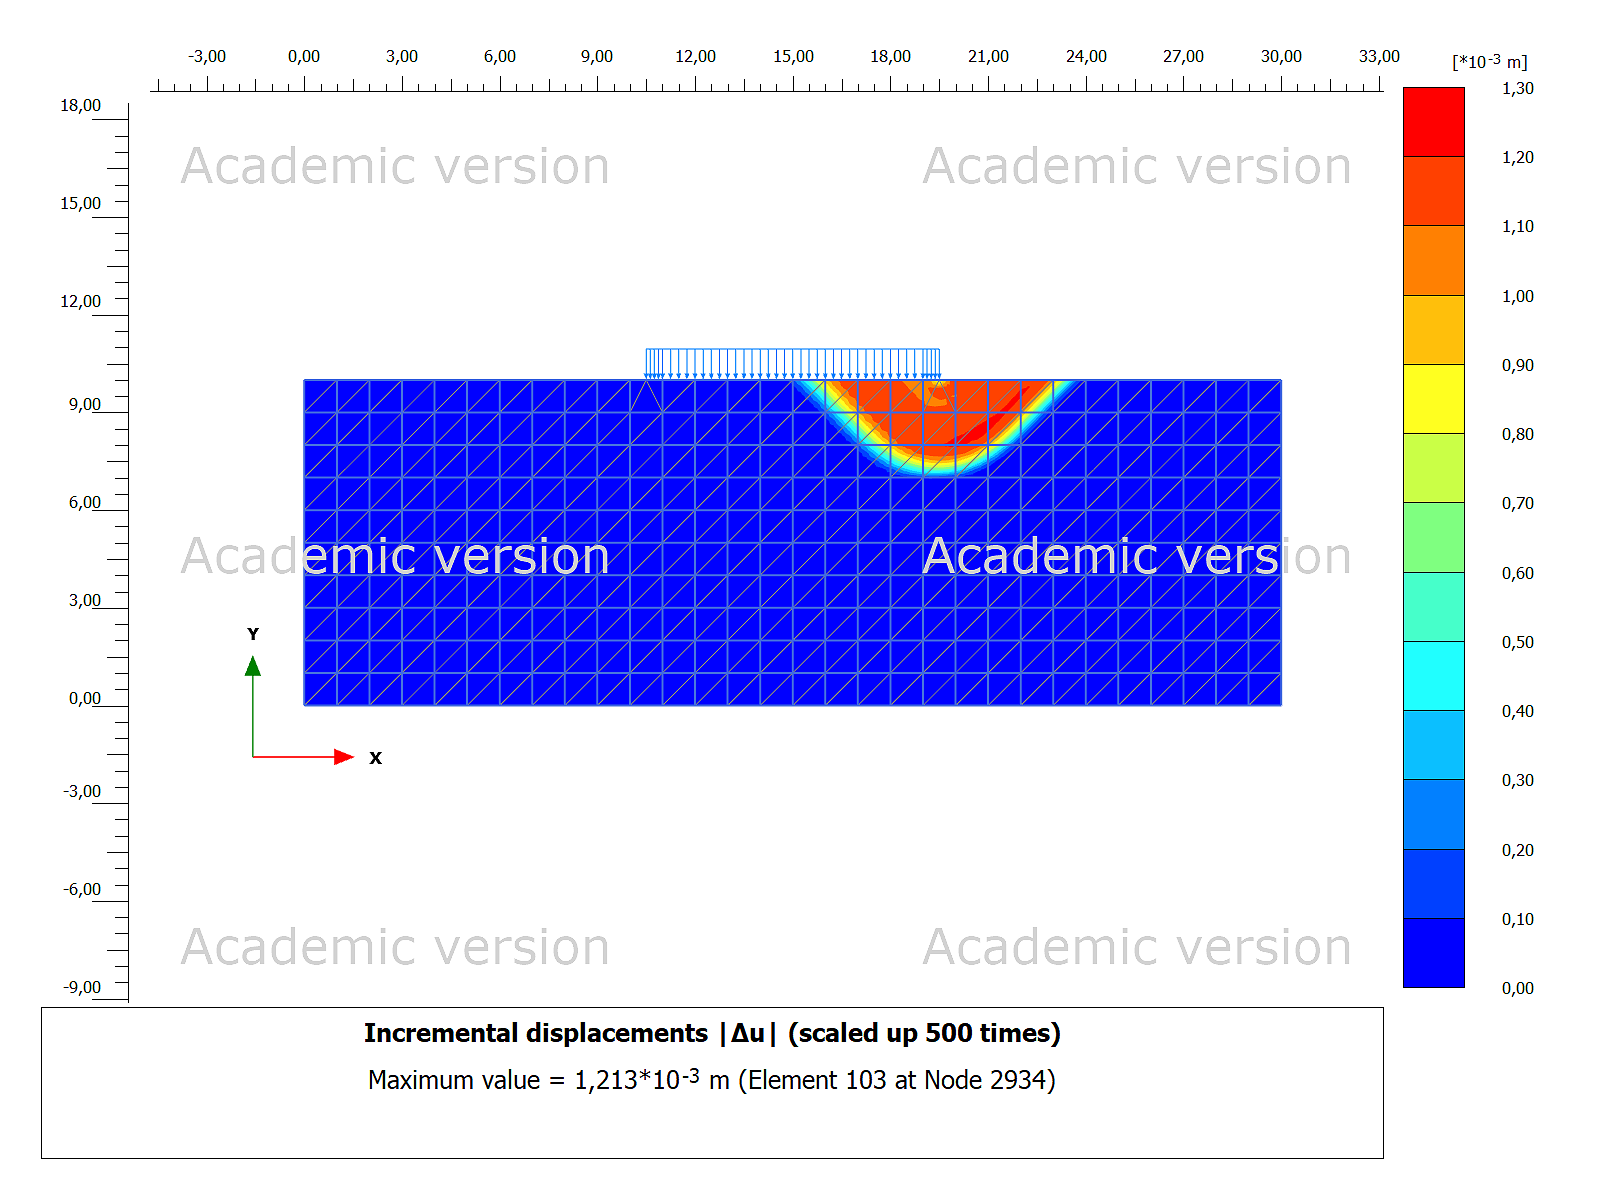
\includegraphics[width=\textwidth]{fig/bc/nx/testutot20211116-1018220.0972879216409623}
    \caption[]%
    {{\small Failure load 97.3 kPa, iteration 201}}
    \label{fig:bc net24}
\end{subfigure}
\vskip\baselineskip
\begin{subfigure}{0.475\textwidth}
    \centering
    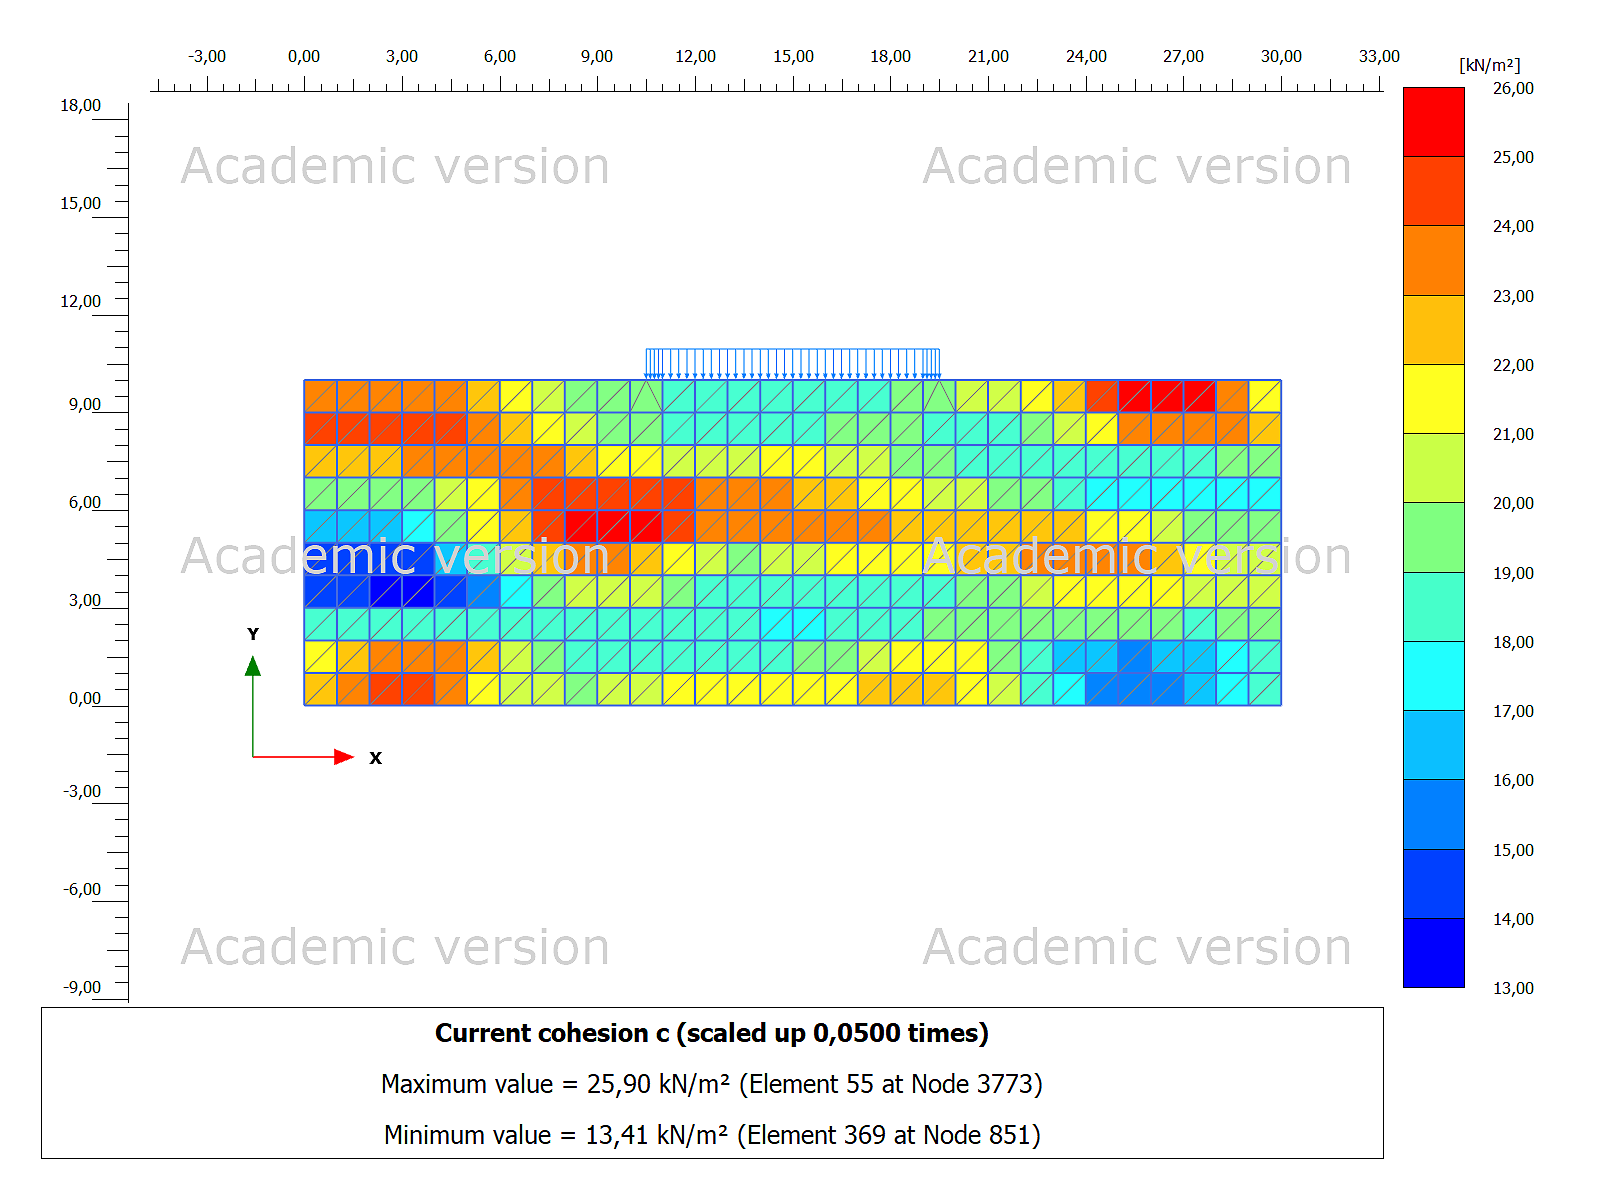
\includegraphics[width=\textwidth]{fig/bc/nx/testp20211116-101338}
    \caption[]%
    {{\small Realization of undrained strength field, iteration 121}}
    \label{fig:bc net34}
\end{subfigure}
\hfill
\begin{subfigure}{0.475\textwidth}
    \centering
    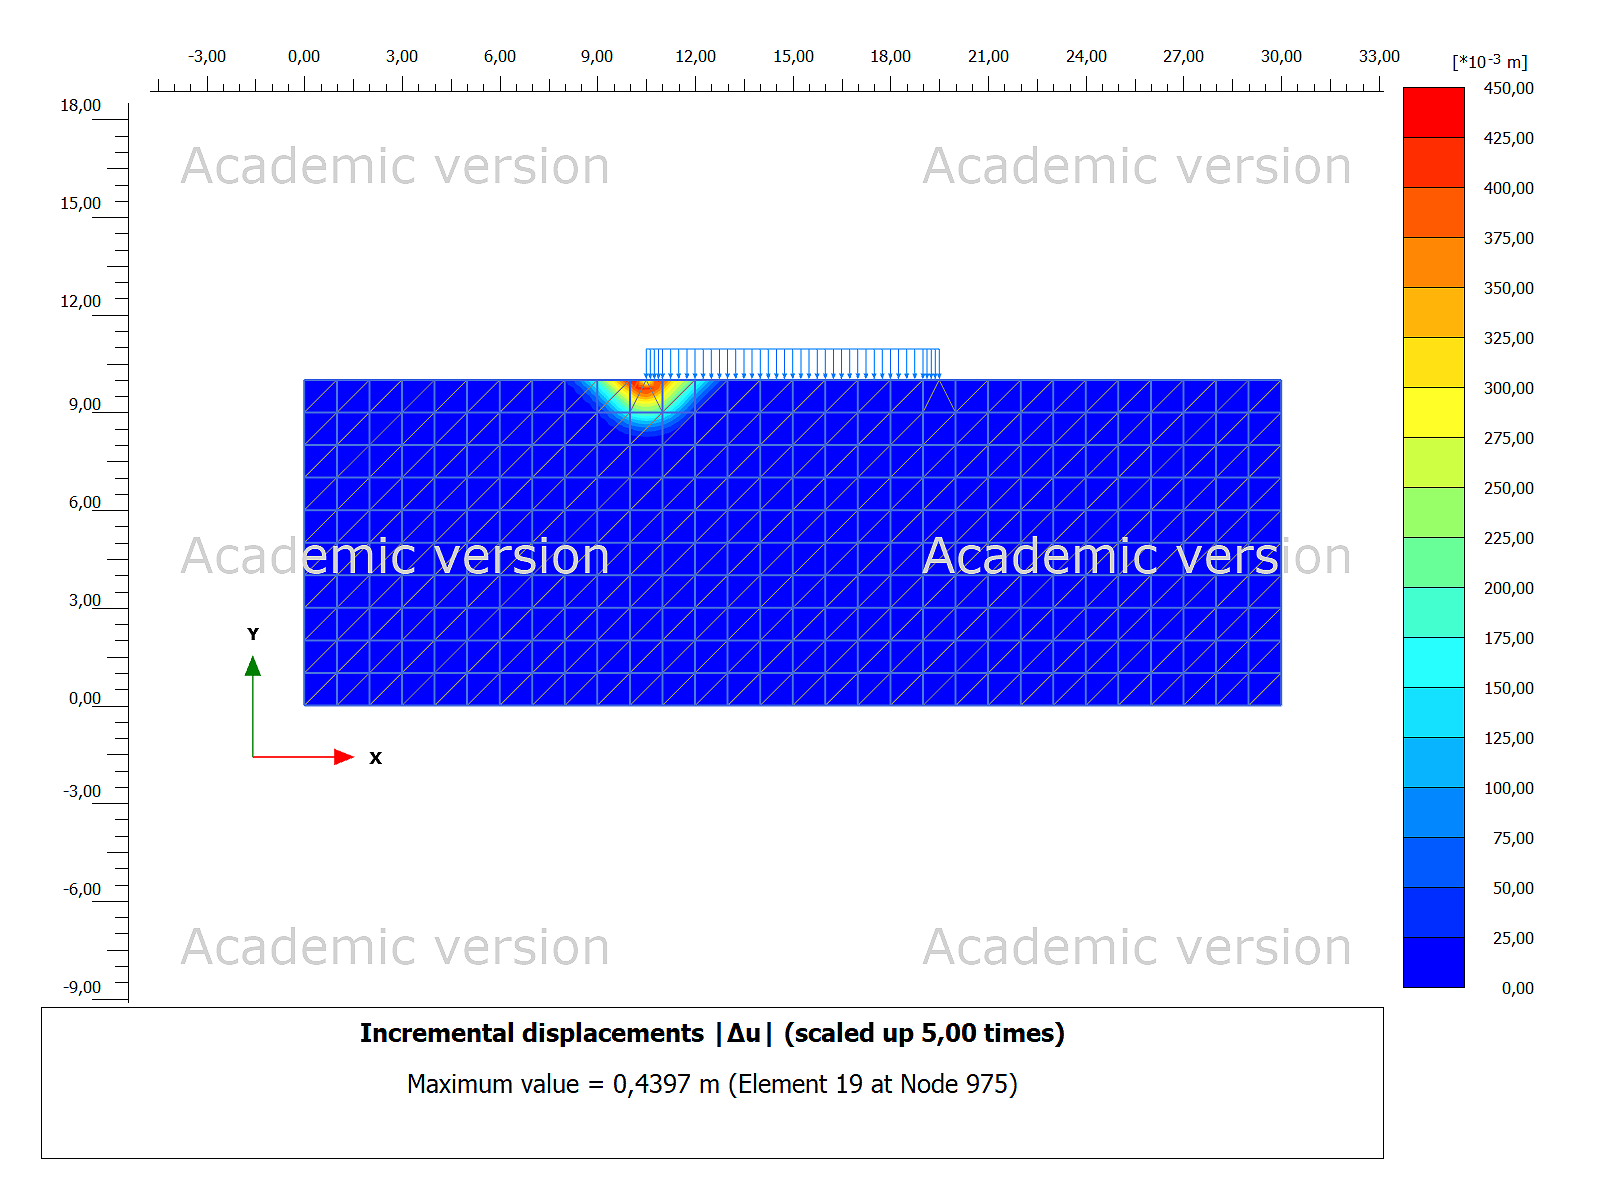
\includegraphics[width=\textwidth]{fig/bc/nx/testutot20211116-1013380.0989476562699225}
    \caption[]%
    {{\small Failure load 98.9 kPa, iteration 121}}
    \label{fig:bc net44}
\end{subfigure}
\begin{subfigure}{0.475\textwidth}
    \centering
    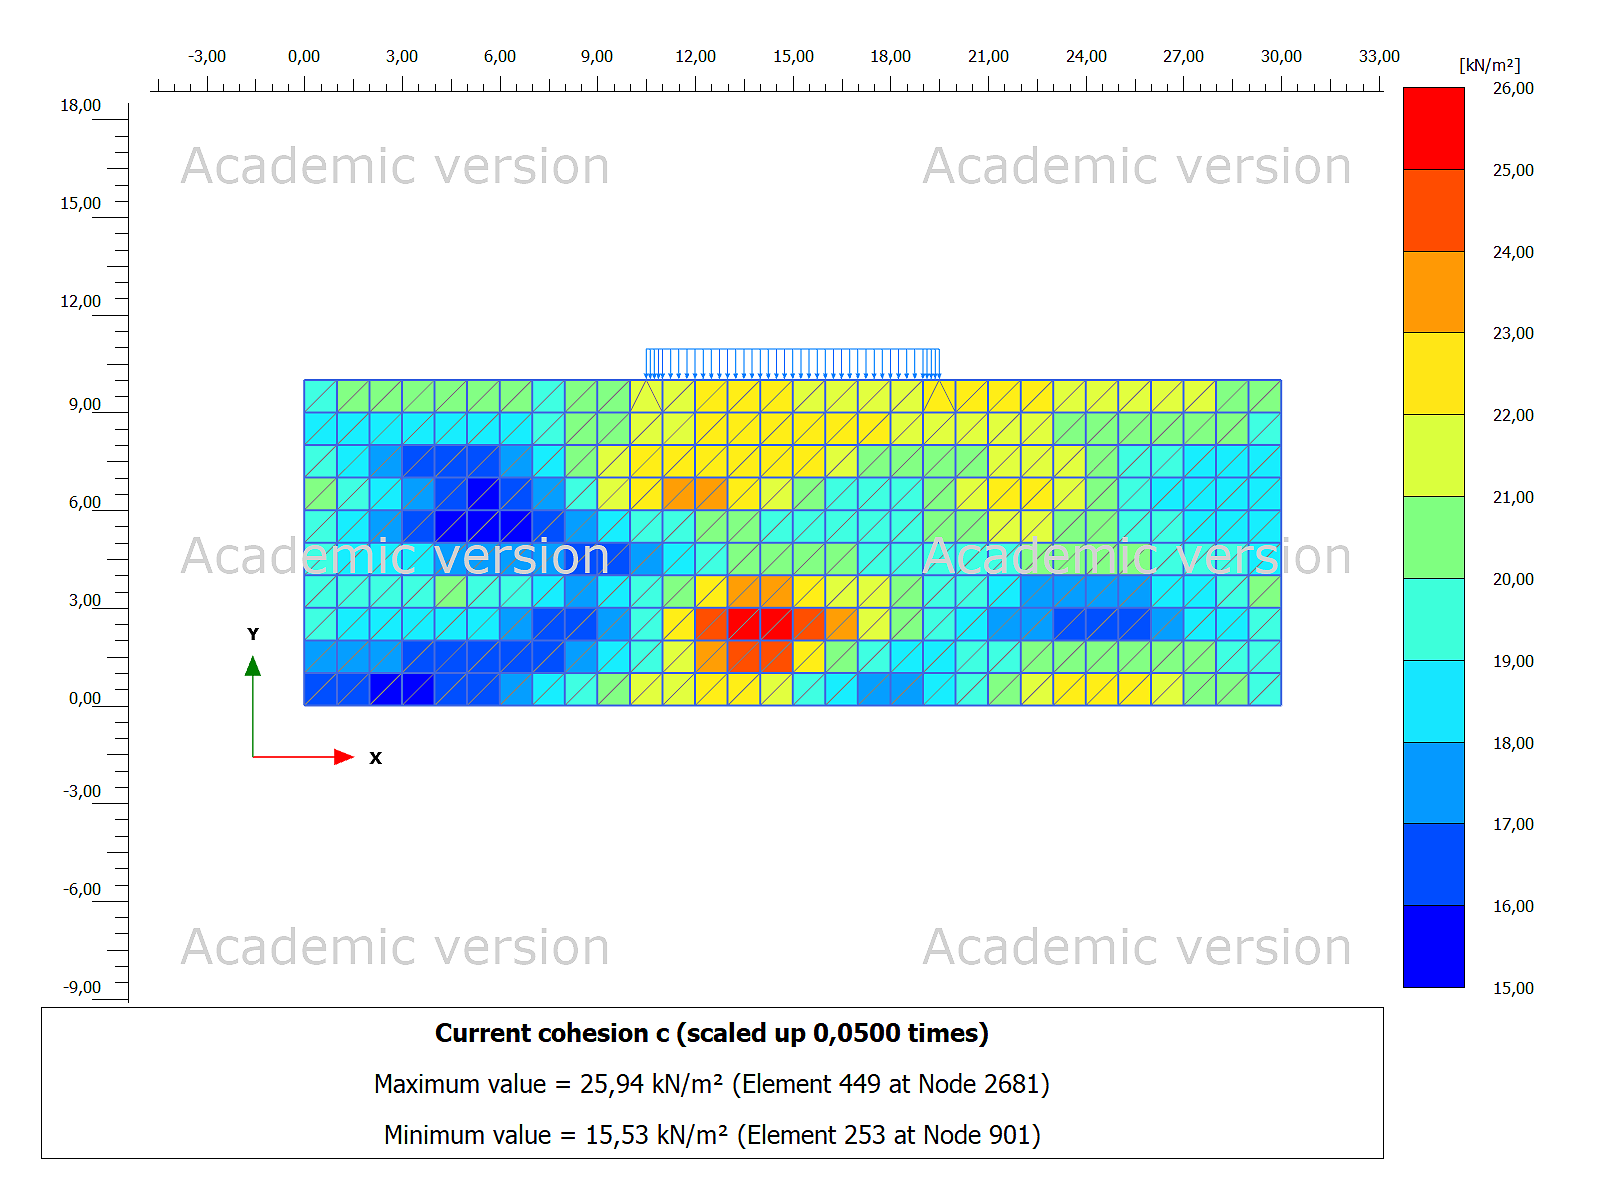
\includegraphics[width=\textwidth]{fig/bc/nx/testp20211116-100901}
    \caption[]%
    {{\small Realization of undrained strength field, iteration 33}}
    \label{fig:bc net56}
\end{subfigure}
\begin{subfigure}{0.475\textwidth}
    \centering
    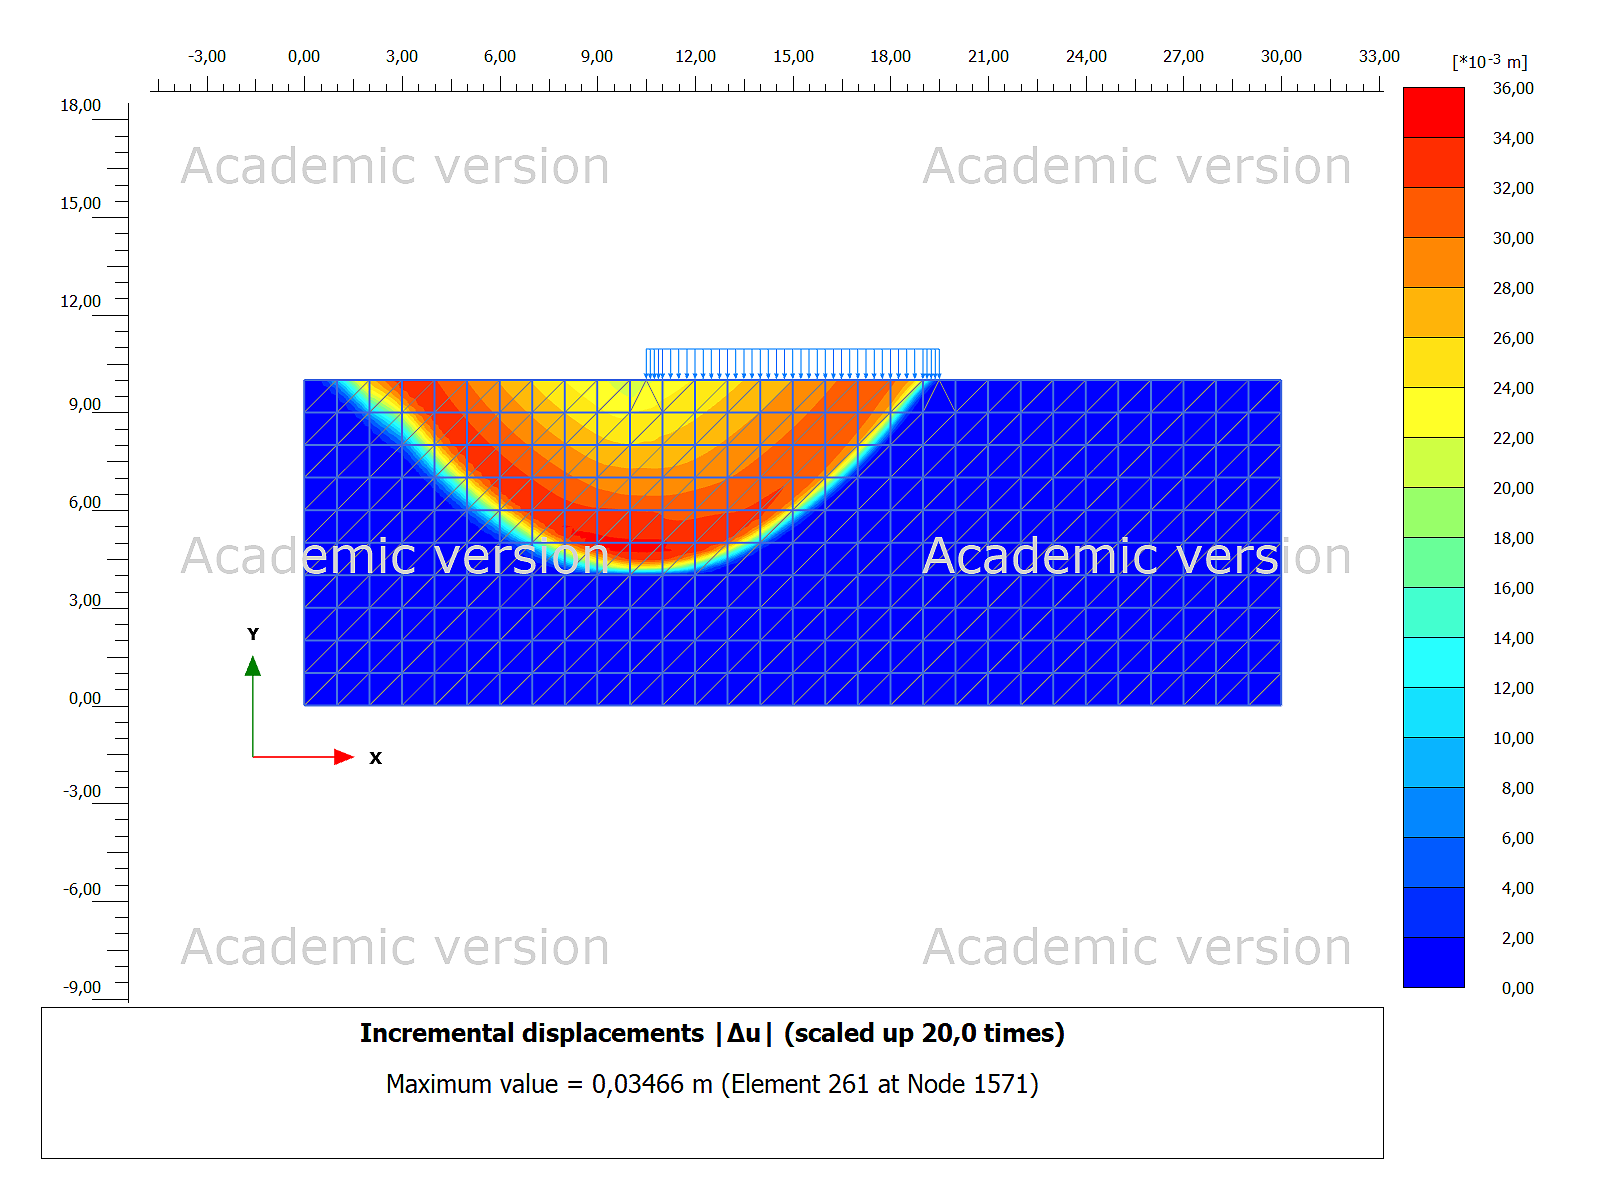
\includegraphics[width=\textwidth]{fig/bc/nx/testutot20211116-100901}
    \caption[]%
    {{\small Failure load 97.6 kPa, iteration 33}}
    \label{fig:bc net66}
\end{subfigure}
\caption[ Three different realizations of random fields created by SRM, their FEM mesh and the failure mechanism after incremental loading.]
	{\small Three different realizations of random fields (Left) created by SRM, their FEM mesh and their corresponding failure mechanism (right) after incremental loading.}
\label{fig:sixbcfields}
\end{figure*}
